\documentclass[oneside]{book}
\usepackage[dvipsnames]{xcolor}
\usepackage{multicol}
\usepackage[top=1in, bottom=1in, left=1in, right=1in]{geometry}
\usepackage{sectsty}
\usepackage[bookmarks=true,bookmarksdepth=subsection]{hyperref}
\usepackage{graphicx}
\usepackage{eso-pic}
\usepackage{changepage}
\usepackage{ifthen}
\usepackage{titlesec}
\usepackage{fancybox}
\usepackage{fancyhdr}
\usepackage{fontspec}
\usepackage{xunicode}
\usepackage{xltxtra}
\usepackage[space]{grffile}

\title{Charms Rewrite}
\date{2016-07-26}
\author{BlueWinds}

\strictpagecheck
\setcounter{page}{250}
\setcounter{chapter}{5}

\newfontfamily\chapfont{Envision}

\pagestyle{plain}
\allsectionsfont{\centering}
\setlength\parindent{0pt}
\setlength\parskip{15pt}
\newlength{\sidewidth}
\setlength{\sidewidth}{6.25in}

\newcommand*{\spelled}[1]{%
  \ifcase#1\or{One}\or{Two}\or{Three}\or{Four}\or{Five}\or{Six}\or{Seven}\or{Eight}\or{Nine}\or{Ten}\or{Eleven}\else\@ctrerr\fi
}

\titleformat{\chapter}[display]{\centering\Large\bfseries}{\chaptertitlename\ \spelled{\thechapter}}{-10pt}{\chapfont\color{MidnightBlue}\Huge\thispagestyle{fancy}}
\titlespacing*{\chapter}{0pt}{0pt}{20pt}
\renewcommand\thesection{}
\titlespacing*{\subsection}{0pt}{0pt}{0pt}

\newcommand{\charm}[6]{
  \parbox{\linewidth}{
    \par \textbf{\color{MidnightBlue}#1}\vspace{2pt} \\
    \ifthenelse{\equal{#5}{-}}{ % No keywords
      \textbf{Cost:} #2; #3 (#4) \\
      \textbf {Prereqs:} #6
    }{ % Has keywords
      \textbf{Cost:} #2 ; #3 (#4) - #5 \\
      \textbf {Prereqs:} #6
    }
  }
  \par
}
\newcommand{\permanentCharm}[2]{
  \parbox{\linewidth}{
    \par \textbf{\color{MidnightBlue}#1} \\
    \textbf {Permanent} \\
    \textbf {Prereqs:} #2
  }
  \par
}

\newsavebox\mysavebox
\newenvironment{sidebarPartial}[2][]{%
   \def\imgcmd{\includegraphics[width=\wd\mysavebox,height=\dimexpr\ht\mysavebox+\dp\mysavebox\relax,#1]{#2}}%
   \begin{lrbox}{\mysavebox}%
   \begin{minipage}%
}{%
   \end{minipage}
   \end{lrbox}%
   \sbox\mysavebox{\fbox{\usebox\mysavebox}}%
   \mbox{\rlap{\raisebox{-\dp\mysavebox}{\imgcmd}}\usebox\mysavebox}%
}

\newenvironment{sidebar}[1]{%
  \begin{figure*}[tb]%
  \begin{sidebarPartial}{resources/bg-sidebar.jpg}{\textwidth}%
  \vspace{6pt}
  \subsection*{#1}\vspace{6pt}%
  \centering
  \begin{minipage}{\sidewidth}
}
{
  \end{minipage}
  \vspace{6pt}
  \end{sidebarPartial}
  \end{figure*}
}

\newenvironment{Ability}[1]{%
  \section{#1}%
  \vspace{-0.25in}\hspace*{-0.75in}\includegraphics[width=8in]{charmTrees/#1.pdf}%
  \begin{multicols}{2}
}
{
  \end{multicols}
}

\pagestyle{fancy}
\setlength\headheight{0pt}
\setlength\headsep{30pt}
\renewcommand{\headrulewidth}{0pt}
\setlength\textheight{659pt}
\setlength\footskip{20pt}
\fancyhf{}
\cfoot{\color{White}\chapfont\thepage}

\begin{document}
  \AddToShipoutPicture{%
    \checkoddpage
    \ifoddpage
      \put(0,0){
\includegraphics[width=\paperwidth,height=\paperheight]{resources/bg-right.jpg}}
    \else
      \put(0,0){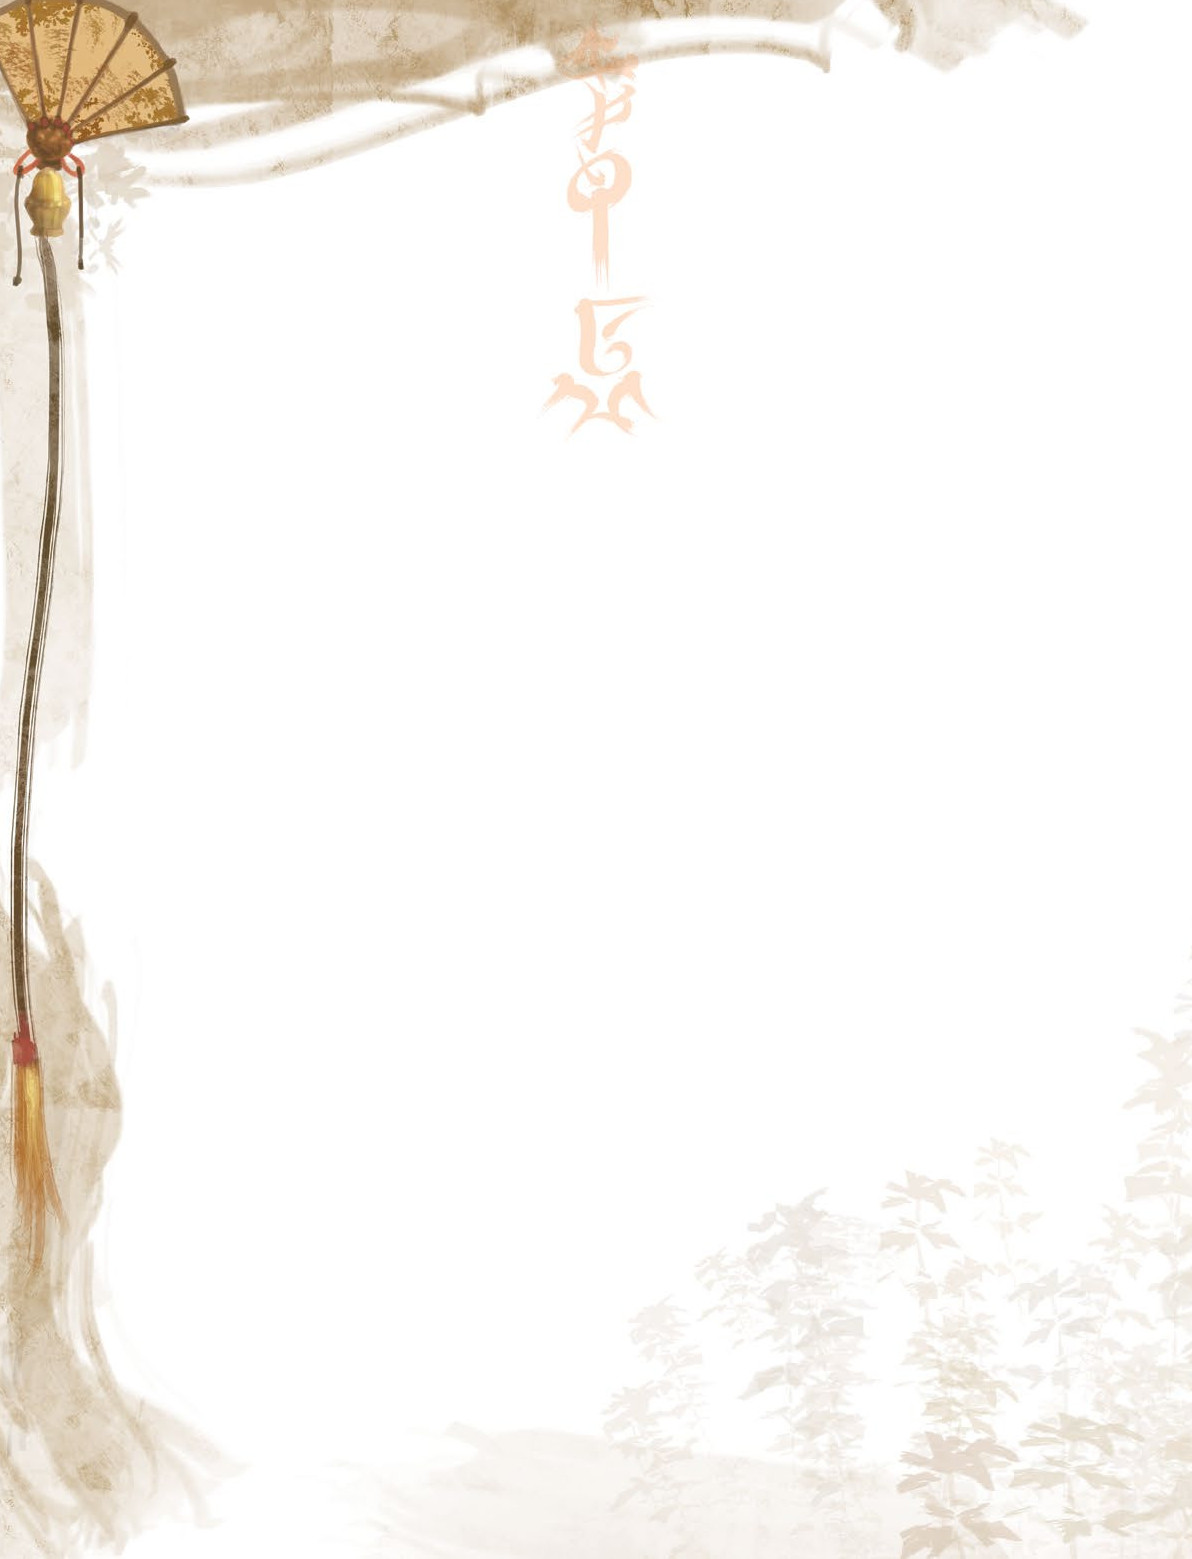
\includegraphics[width=\paperwidth,height=\paperheight]{resources/bg-left.jpg}}
    \fi
    \put(292,19){
\includegraphics[width=0.42in]{resources/bg-page-num.png}}
  }

\chapter{Charms}
\begin{multicols}{2}

The Exalted are mighty. Some break swords upon their skin or shatter stone with their fists while others sing songs that move the rocks themselves to tears. As they grow into the fullness of their power, they may form new reality out of primordial chaos, single handedly rout armies or step through shadows and minds in search of secrets

\par These powers and more are represented as Charms, tidy little packages of name, flavor and mechanical effect the game wraps around your character's supernatural prowess. This abstraction is just that - an abstraction. Simply put, we talk about Charms as power and magic and techniques, but when a player has her character use Monkey Leap Technique, the Solar leaps high enough to clear a rooftop - but the character is simply applying their skill at athletics. Charms aren't magic spells. Those who behold a Solar throwing aside a boulder would remark on her incredible strength, but not her use of Increasing Strength Exercise or Thunder's Might.

\end{multicols}
\section{Reading charms}
\begin{multicols}{2}

\subsection*{Minimums}
\par Solar charms all require a minimum level of skill in their associated ability, and many of them expand on earlier charms in that ability. A character must meet all of a charm's Prereqs before she can learn it. Some charms offer also repurchases - by buying a charm additional times, a character can unlock further power.

\par A Solar treats her Essence as 5 for charms in her Supernal Ability for the purposes of prerequistes, upgrades and accessing repurchases, but not for calculating numeric effects (such as range or number of successes added).

\subsection*{Costs}
\par Most charms have a cost - they require an exertion of motes, willpower, initiative or even health levels. A character must pay the full cost before activating a charm - they cannot spend their initiative below 0, for example.

\begin{tabular}{ll}
  Example & Cost\\
  \hline
  3m, 1wp & 3 motes, 1 willpower\\
  2i & 2 initiative\\
  1hl & 1 bashing health level\\
  2lhl & 2 lethal health levels\\
  1ahl & 1 aggravated health level\\
\end{tabular}

\subsection*{Types and Timing}
\par Charms come in one of four types, which explain when and how they can be activated.

\begin{itemize}
\item Permanent: A permanent Charm is just that - a permanent enhancement to the character's prowess, costing nothing to enjoy and providing its benefits passively at all times.
\item Simple: A simple Charm counts as a combat action in and of itself, and cannot be placed in a flurry. Some take longer, as specified in their text.
\item Reflexive: Reflexive Charms can be activated either before or after other actions, including between the actions of a flurry or multi-attack charm, but not in the middle of an action. Many of them list specific triggers - a charm may be used only once per triggering event.
\item Supplemental: Supplemental Charms enhance an action or defense, such as an attack roll, whole craft project, or an attempt to dodge an attack. They are activated during an action - usually while it's being declared, but sometimes latter in the process of resolving it (as specified by the individual charm).
\end{itemize}

\par Any number of supplemental charms may apply to a single roll or defense, but a solar cannot activate the same Charm on the same action multiple times. Supplemental charms may be used to aid actions or defenses even if the character isn't aware of making them - she can use her charms to enhance an Awareness roll to notice danger, or defend herself with Integrity charms even while asleep, unconscious or drugged, for example.

\begin{sidebar}{Conflict}\
  \par When they directly affect another character, players (including the Storyteller) must openly declare and charms they're using and their effects. The majority of charms must be used before a dice roll is made (Post-Roll charms are obviously an exception!), and the active character declares first in the case of an opposed action. Below is a detailed breakdown of who can use what when, but don't be intimidated - very seldom do you need to step through all of these out loud.

  \begin{enumerate}
    \item A player declares their action and activates any reflexive or supplemental charms related to it.
    \item If the action is against another character, that character's player activates any reflexive or supplemental charms to boost their defense.
    \item The active player rolls, and activates any Post-Roll charms they wish to use.
    \item The defending player activates any Post-Roll charms.
    \item Resolve the action. An attack might hit (triggering a damage roll, and possibly more post-roll charms related to damage) or miss, or a character might be subject to social influence and have the option to spend wp to resist.
    \item Both players may activate any reflexive charms triggered by the action - to counterattack, regain motes, etc.
  \end{enumerate}
\end{sidebar}

\subsection*{Duration}
\par After their type, non-permanent charms list a duration in parentheses. The charm's effects continue to apply and its mote cost remains committed until it ends (those motes cannot be regained until the charm ends). Long-running charms can be ended reflexively at any time, even while the character is unconscious or asleep.

\begin{itemize}
  \item Instant: Instant charms have their effect - often on a single action or roll - and then they're done.
  \item One Round: The charm lasts until the start of the character's next combat action.
  \item One Scene: The charm lasts until the scene changes (see pg. 184).
  \item Indefinite: The charm remains on as long as the character desires (even while sleeping or unconscious).
\end{itemize}

\subsection*{Keywords}
\par Some charms list one or more keywords after their duration.

\begin{itemize}
  \item Advantage: A charm with this keyword can only be used against an opponent with less initiative than the Solar.
  \item Attack-action: Using this charm counts as the Solar's attack action for the round. She may not use it if she's already taken one this round (or activated another Attack-action charm).
  \item Counterattack: This charm may not be used in response to attacks created by other charms with the Counterattack keyword, and only one Counterattack charm may be activated for a given trigger. Attacks it creates cannot be Clashed, even with the use of charms.
  \item Form: A character may only have one Form charm active at a time. Ending one form charm to activate another immediately refunds all motes committed to the first form.
  \item Group: Any rolls this charm supplements or creates ignore the penalty for group group social influence.
  \item Iconic: This charm may only be activated when the Exalt's anima is at the Bonfire / Iconic level.
  \item Mute: This charm's cost does not add to the Exalt's anima level unless she wants it to.
  \item Perilous: Charms with this keyword cannot be used in Initiative Crash. If the charm lasts longer than Instant, it ends if the Exalt crashes.
  \item Once/X: A character can only use this once per scene/day/story/season.
  \item Pilot: To activate charms with this keyword, the character must be the helmsman or captain of a vessel. For Sailing related charms without it, "the character's ship" refers to any vessel she's a passenger, crew, or otherwise associated with.
  \item Post-roll: This charm is activated after dice have been rolled, but before success has been determined. For example, a player could wait until she knows how many successes have been rolled on an attack before activating a Post-roll defense.
  \item Psyche: A power with this keyword is an unnatural, hypnotic, or sorcerous power that magically influences, controls, or cripples an opponent's thoughts or feelings.
  \item Quickshot - Attacks granted or enhanced by this Charm do not require an Aim action to succeed, regardless of range.
    This Charm's effects can stack.
\end{itemize}

\end{multicols}
\section*{Limitations and Terminology}
\begin{multicols}{2}
\par A Solar may not add more than (Attribute + Ability) dice to a single roll, and each automatic success counts as two dice. If a combination of charms would add more dice/successes than that, discard the extras.
\par Some charms grant the character a "full excellency." This is shorthand for "add (Attribute + Ability) dice to the roll".

\par  When charms refer to increasing of decreasing a duration in increments, use the following chart: \\
    Decades --- Years --- Months --- Weeks --- Days --- Hours --- Minutes --- Seconds

\par Charms can modify dice rolls in a variety of ways. Some of these are also mentioned in the glossary, but repeated here for ease of reference. If multiple effects modify a single roll, apply them in this order.
  \begin{enumerate}
    \item Add X dice: Roll X more dice than you normally would.
    \item X automatic successes: After rolling, add X successes.
  \end{enumerate}

\begin{sidebar}{Multiple Attacks}
If a charm asks the solar to divide her initiative up evenly into some number of attacks, divide as evenly as possible. For example, if she were dividing 8i among three attacks, she'd make attacks with 3i, 3i and 2i.
\par\vspace{6pt} If any effect would cause her to crash in the middle of a multiattack (a counterattack or dodge charms sapping her initiative, for example), she crashes immediately and cannot make any more attacks. After all attacks complete, if she isn't crashed:
\begin{itemize}
  \item If she hit with at least one decisive attack, she resets to base initiative.
  \item If all her decisive attacks missed, she loses initiative as though she'd only missed with one.
\end{itemize}
\par\vspace{6pt} If a charm applies a single attack against multiple opponents, apply the attack to all opponents before anyone activates Reflexive effects based on it.
\begin{itemize}
  \item If she hits at least one opponent with a decisive attack, she resets to base initiative.
  \item If she missed all opponents with a decisive attack, she loses initiative for missing with a single attack.
\end{itemize}
\end{sidebar}

\end{multicols}
\section*{Excellencies}
\begin{multicols}{2}
\par The Chosen enjoy a fundamental power called the Excellencies. When a Solar uses an Excellency, she channels pure Essence into her endeavors - the fundamental power of the sun quickens and strengthens her blows, sharpens her sight, or steadies her hands.

\par Solars automatically gain an Excellency for each Caste and Favored Ability in which they possess at least one dot, as well as any Ability for which they have learned at least one Charm.

\charm{Excellent Solar (Ability)}
{1m per die, or 2m per +1 to static value}
{Supplemental}
{Instant}
{-}
{(Ability) 1}
The Solar adds +(motes spent) dice to an (Ability) roll, or +(motes spent / 2) to a static value derived from (Ability). Remember “Using Charms and Charm Limitations” above.
\end{multicols}

\begin{Ability}{Archery}

  \charm{Sight Without Eyes}
  {1m}
  {Supplemental}{Instant}{-}
  {Archery 3}
  This charm supplements an Archery attack, allowing the Exalt ignores all penalties for visual conditions. Smoke, fog, and pitch darkness don't hinder her, though other factors such as high winds and cover still apply against the attack.

  At Archery 5+, Essence 3+, she can momentarily see through cover, perceiving her targets as silhouettes the colors of bright anima.

  \charm{Force Without Fire}
  {3m}
  {Supplemental}{Instant}{-}
  {Archery 4, Sight Without Eyes}
  This charm supplements a withering Archery attack from short or close range. If the attack does at least as one damage as her target's Stamina, that Initiative is lost rather than transferred to the Solar, and the target is knocked down and back an entire range band.

  \charm{There Is No Wind}
  {3m}
  {Supplemental}{Instant}{-}
  {Archery 5, Essence 2, Sight Without Eyes}
  This charm supplements an Archery attack, allowing it to be made from up to extreme range. The Solar also ignores penalties from non-visual conditions such as high winds, bad weather, flawed ammunition, and so on (but not cover).

  If the attack is withering, her accuracy is calculated as if it were made from short range regardless of the distance she's firing from.

  \charm{Phantom Arrow Technique}
  {1m}
  {Supplemental}{Instant}{-}
  {Archery 3}
  This charm supplements an Archery attack, allowing the Exalt to shoot without ammunition.

  At Essence 3+, once per scene she may pay an additional 1wp. An arrow so infused cannot be destroyed or pulled from the target as long as she lives. A tree can still be cut down, a wall still reduced to rubble - but the arrow will remain inviolate. Only the Solar who fired this arrow, or one blessed with her permission, may remove it from its resting place.

  \charm{Immaculate Golden Bow}
  {5m, 1wp}
  {Simple}{One Scene}{-}
  {Archery 4, Essence 2, Phantom Arrow Technique}
  The Exalt creates a weapon from her anima with stats identical to a powerbow or other artifact Archery weapon. It glows like a torch. Players may add custom Evocations to Immaculate Golden Bow as they would another artifact weapon, working with their Storyteller to create Evocations that fit the character's personality or iconic anima manifestation.

  \charm{Fiery Arrow Attack}
  {2m}
  {Supplemental}{Instant}{-}
  {Archery 4}
  This charm supplements a Decisive Archery attack, causing the arrow to explode in a spectacular flare that can be seen for miles. Every target using shadows for cover within two range bands must roll Stealth with a -2 success penalty or be revealed.

  \charm{Shadow-Seeking Arrow}
  {3m, 2i}
  {Reflexive}{Instant}{Quickshot}
  {Archery 5, Essence 3, Fiery Arrow Attack}
  During combat, if the Lawgiver's Awareness check uncovers an opponent, she may immediately make a withering or decisive Archery attack against that opponent. She may pay to use this Charm against each opponent, if she uncovers more than one with a single Awareness check.

  \charm{Trance of Unhesitating Speed}
  {4m, 1wp}
  {Simple}{Instant}{Quickshot, Perilous}
  {Archery 3}
  The Exalt makes up to (Lower of Dexterity or Initiative/3) decisive Archery attacks, dividing her initiative evenly between them. Each 10 she rolls on an attack increases the base damage of that attack by one.

  \charm{Arrow Storm Technique}
  {5m, 1wp}
  {Supplemental}{Instant}{-}
  {Archery 5, Essence 2, Trance of Unhesitating Speed}
  This charm supplements a Decisive Archery attack. In addition to its initial target, it strikes up to (Essence * 3) targets up to medium range from the initial one using the same attack roll, but dividing her initiative evenly among all attacks. Each one then gains (Perception) raw damage.

  \charm{Revolving Bow Discipline}
  {6m, 1wp}
  {Simple}{Instant}{Perilous}
  {Archery 5, Essence 3, Arrow Storm Technique}
  The Solar makes a withering Archery attack against a single uncrashed target within short or close range. If it hits she may make another, repeating until she either misses or crashes her opponent (or it loses a point of magnitude if it's a Battle Group).

  \charm{Heavens Crash Down}
  {6m, 2i, 1wp}
  {Reflexive}{Instant}{-}
  {Archery 5, Essence 4, Revolving Bow Discipline}
  This charm may be used when the Solar is in her -4 health levels and targeted by a withering attack from short or close range. She Clashes the attack using Archery, with (Essence) automatic successes. If she wins the clash, Initiative she would gain is instead rolled as dice of decisive damage against her target, ignoring hardness and doubling 10s.

  An Essence 5+ repurchase of this Charm allows the Solar to spend Initiative she doesn't have, going into (or deeper into) the negative.

\end{Ability}

\begin{Ability}{Athletics}

  \charm{Graceful Crane Stance}
  {3m}
  {Reflexive}{One Scene}{-}
  {Athletics 1}
  The Exalt has perfect balance, and can stand or run on things too narrow or weak to support her normally, with no chance of falling or breaking through. She automatically succeeds at the (Dexterity + Athletics) roll for such feats as running on a guy wire, standing on a crumbling parapet, balancing on the tip of a pine tree, and similar.

  \charm{Feather Foot Style}
  {3m}
  {Supplemental}{Until the Exalt stops running}{Mute}
  {Athletics 3, Graceful Crane Stance}
  This charm supplements a move action, allowing the Exalt to dash over liquid or unstable surfaces as if they were solid and move over surfaces as thin as rice paper without breaking through. She may also move across lava or other dangerous surfaces without getting hurt. As long as she is moving at a quick pace, she need not pay the activation cost again.

  At Essence 2+, she can pause on unstable surfaces without breaking through, changing the duration of this Charm to “one stunt.” She can walk slowly across the surface of a still pond, pause on the crumbling parapet of a castle to give a speech, and so on. This mode does not protect against hazardous surfaces.

  \charm{Spider Foot Style}
  {3m}
  {Reflexive}{Essence + 1 Turns}{Mute}
  {Athletics 4, Feather Foot Style}
  The Solar can run up walls, stand upside down on horizontal surfaces such as tree branches, bridge bottoms or overhangs, lay flat against a ceiling looking down at her prey, or other similar feats.

  \charm{Monkey Leap Technique}
  {2m}
  {Supplemental}{Instant}{-}
  {Athletics 2}
  This charm supplements a reflexive Move action, allowing the Solar to leap forward or straight up one range band. A Solar using this Charm can easily leap to the top of a twenty foot wall or cross a Nexus street over rooftops without a roll. If the Solar continues to leap each turn the cost is reduced to 1m after the first activation.

  \charm{Soaring Crane Leap}
  {2m}
  {Reflexive}{One round}{-}
  {Athletics 3, Monkey Leap Technique}
  When falling, the Exalt may activate this charm to drop only a single range band until her next turn. In order to survive a very long falls without damage, she must use for at least two rounds before touching the ground. The Exalt can also use this Charm to drift long distances through the air as she continues to fall. If she was moving forward when the fall began, she may continue to move in that direction on future rounds, falling downward one range band for each band of forward motion.

  \charm{Mountain-Crossing Leap Technique}
  {7m, 1wp}
  {Simple}{Until she stops leaping}{-}
  {Athletics 5, Essence 3, Soaring Crane Leap}
  The Exalt makes a leap three up to four range bands forward or three straight up. This Charm stays active every turn until the Solar stops leaping across range bands, making it possible for the Exalt to cross a mountain in minutes.

  This charm may not be activated with opponents at Close range, but as an exception to the normal Simple charm rules, may be flurried with Disengage.

  \charm{Leaping Tiger Attack}
  {4m, 1wp}
  {Supplemental}{Instant}{Advantage}
  {Athletics 5, Essence 2, Thunderbolt Attack Prana}
  This charm supplements a non-ranged attack, allowing her to immediately move Close from up to medium range. Using it replaces her normal reflexive Move action for the round. If her attack is withering, it doubles damage dice after soak. If decisive, it adds her Essence score to the base damage of the attack.

  \charm{Increasing Strength Exercise}
  {3m or 3i per bonus}
  {Simple}{One Scene}{-}
  {Athletics 3}
  For every three motes of Essence or Initiative the Exalt spends, she raises the base damage of her withering and decisive attacks by one and lowers the minimum Strength of all Feats of Strength by one. She also adds that many dice to all Strength-based rolls. She cannot spend more than (Essence * 3) motes or initiative in this way.

  \charm{Legion Aurochs Method}
  {6m}
  {Supplemental}{Instant}{-}
  {Athletics 5, Essence 3, Thunder's Might}
  This charm supplements feats of strength. Add 50% to the Solar's rolled successes (round down).

  \charm{Nine Aeons Thew}
  {1m, 1wp}
  {Supplemental}{Instant}{-}
  {Athletics 5, Essence 5, Legion Aurochs Method}
  This charm supplements a feat of strength, reducing its difficulty by (Solar's Essence + 2), and she counts as meeting its Strength prerequisite no matter how high that requirement might be.

  \charm{Racing Hare Method}
  {5m, 1wp}
  {Reflexive}{One Hour}{-}
  {Athletics 4, Essence 2, Lightning Speed}
  This charm may be used any time outside of combat. The Lawgiver travels overland as fast as a running horse. If she renews this technique at the end of an hour, ignore the Willpower cost.

  \permanentCharm{One Extra Step}
  {Athletics 5, Essence 4, Godspeed Steps}
  Once per scene, the Exalt may take a second move action on her turn.

\end{Ability}

\begin{Ability}{Awareness}

  \permanentCharm{Keen Sense Technique}
  {Awareness 3, Sensory Acuity Prana}
  When the Solar purchases this charm, choose Sight, Hearing, or Smell, Taste and Touch.

  The Solar gains three dice on any Awareness roll involving the chosen sense(s).

  With an Essence 2+ repurchase, she chooses a second sense.
  With an Essence 3+ repurchase, the bonus applies to all the listed senses. In addition, the Solar takes no penalty to rolls because of being blind or deaf. If both, she only takes -2 on tasks that would normally require those senses.

\begin{sidebar}{What can I do with Awareness?}
  In addition to the obvious use of noticing assassins, a Solar with 5 successes on an Awareness roll might:

  \begin{itemize}
    \item Read a letter at a glance from across the room, quickly count masses of troops, see through smoke and fog.
    \item Identify an individual by scent, count the number of individuals in a crowded room, detect poison before taking a bite of food, identify every ingredient in a stew, tell how long ago a specific person left a room.
    \item Listen to conversations through thick stone walls, identify materials by touch, recognize counterfeits, feel an earthquake minutes or hours before it happens.
  \end{itemize}

  With 10 successes, she might:
  \begin{itemize}
    \item Spot a field mouse a quarter mile, read a letter at a hundred yards, critique the mating habits of insects.
    \item Smell blood from a mile away, identify which farm food came from by tasting each field in turn
    \item Listen in on a whispered conversation out to long range on a battlefield, read by tracing her fingers over the ink on a page, orient herself to the exit in complete darkness.
  \end{itemize}
\end{sidebar}

  \charm{Genius Palate Summation}
  {2m}
  {Simple}{Instant}{-}
  {Awareness 4, Essence 2, Keen Sense Technique (Smell, Taste and Touch) or Keen Sense Technique x3}
  This Charm acts as an automatically successful read intentions action to determine the emotional state of the one who prepared a meal or poured a drink. The Solar need only sample a single bite of a meal or take a single sip of a drink to gain this understanding.

  \charm{Foe-Scenting Method}
  {3m}
  {Simple}{Instant}{-}
  {Awareness 5, Essence 2, Keen Sense Technique (Smell, Taste and Touch) or Keen Sense Technique x3}
  The Solar makes a scent-based Read Intentions actions using (Perception + Awareness) to determine a target's disposition, out to medium range without the need to directly interact.

  \charm{Rumour Of The Earth}
  {5m, 1wp}
  {Simple}{Instant}{Mute}
  {Awareness 5, Essence 2, Keen Sense Technique (Hearing) or Keen Sense Technique x3}
  The Lawgiver places her head against the ground and listens for five minutes. She can hear any creature larger than a mouse moving within (Essence * 5) miles, and learns their general location, number, and speed and direction of movement. Used in a city or other busy area, the results may not be that useful, but will still indicate any general motion of large numbers of people.

  \charm{Unsurpassed Hearing Discipline}
  {5m, 1wp}
  {Simple}{One conversation}{-}
  {Awareness 5, Essence 3, Keen Sense Technique (Hearing) or Keen Sense Technique x 3}
  The Solar listens in on conversations that happened in her location up to (Essence x 5) hours prior to her arrival as though it were happening right next to her. She must sit still and listen intently for as much of the conversation as she wishes to hear.

  \charm{Dedicated Unerring Ear}
  {3m}
  {Reflexive}{One exchange}{-}
  {Awareness 5, Essence 4, Unsurpassed Hearing Discipline}
  This charm may be activated any time the Exalt is addressed by someone for whom she holds a Major or Defining Intimacy, no matter how far away he is. So long as she's on the same plane of existence, the Solar can hear the words clearly, as if they were in the same room, so long as they are addressing their speech to her. She can hear everything her compatriot wishes to say to her, until the character has been silent for ten seconds or longer.

  With an Essence 5 repurchase, the charm may also be activated whenever any character uses the Solar's name to refer to her, even if they are not addressing her, without the need for a relevant intimacy. If her name is in common use, the Storyteller should still mostly call attention to interesting and relevant references she might overhear, rather than mundane conversations.

  \permanentCharm{Curse-Catching Instinct}
  {Awareness 3, Essence 2}
  Whenever another character lays a curse upon the Solar or meddles with her fate, she rolls (Perception + Awareness), difficulty (meddler's Essence). Success lets the Solar know vaguely what happened (someone is meddling with your fate). With 3 threshold successes she learns a summary of what happened (Sidereal Astrology associated with The Sword is being used to make you more likely to fall ill). With 5 threshold successes she learns what happened in detail (Tekkip Nannaja, Chosen of Endings, is using Astrology associated with The Sword to increase the TN of your disease-resistance rolls to 9 until Calibration).

  \charm{Vigilant Friend Technique}
  {1m}
  {Simple}{Indefinite}{Stackable}
  {Awareness 4, Essence 2, Curse-Catching Instinct}
  The Solar touches a willing character. As long as she keeps the mote committed, she may roll (Perception + Awareness) to notice danger to the character, as though she were standing next to him. Add +1 difficulty if he's more than 1 mile away from her, +2 if more than 10, +3 if more than 100, +4 if he's anywhere on the same plane of existence or +5 if he's not. She doesn't learn the form of the danger, only that it exists, a general sense of the severity, and his location.

  If the character dies, the Solar automatically notices and knows where it happened.

  \permanentCharm{Surprise Anticipation Method}
  {Awareness 3}
  The Solar takes no penalties to Awareness rolls to notice personal danger from being tired, asleep or unconscious. She wakes with a premonition of danger (though not its source) even if she fails such a roll.

  In addition, for every 10 the Solar rolls on an Awareness check to notice or locate a hidden enemy, trap, or any source of harm not readily apparent, she gains 1m.

  \charm{Vigilant Warrior's Counterstroke}
  {5m}
  {Reflexive}{Instant}{Once/Scene}
  {Awareness 5, Essence 3, Surprise Anticipation Method}
  The Solar may use this charm when targeted by a Surprise or Ambush attack. She may draw a weapon, then Clashes the attack. If clashing an Ambush she suffers -2 on her roll.

  \permanentCharm{Uncanny Perception Technique}
  {Awareness 2}
  When in the presence of dematerialized spirits, sorcerously-crafted living shadows and other generally invisible or intangible subjects, the Solar experiences strange sensory phenomena appropriate to the nature of the being, such as the sound of bells, the scent of chill winter wind or a coppery taste. She automatically notices the presence of such beings (but not their location) unless they hide from her using Stealth. These sensations are as distinctive as a voice - she'll almost always recognize a spirit or being she's met before.

  \charm{Eye of the Unconquered Sun}
  {10m, 1wp}
  {Simple}{One round}{-}
  {Awareness 5, Essence 4, Surprise Anticipation Method, Uncanny Perception Technique}
  The Solar's caste mark blazes like a tiny sun, cancelling any Essence-muting magic the Solar may be using and removing her from stealth. She applies a single Perception + Awareness roll with (Essence) bonus dice against every character's Evasion out to long range. Even solid walls are no protection. Any character who didn't dodge is subject to the following effects.

  \begin{itemize}
    \item They automatically know they've been spotted, and by who.
    \item All magical and mundane Stealth effects are canceled, and she becomes aware of their presence.
    \item Fog lifts, smoke parts, and clouds dissolve.
    \item Dematerialized spirits are forced to materialize, paying full cost of the Materialize Charm or as much of it as they can pay.
    \item All disguise magic is stripped. Mundane disguises tatter and melt away, shapeshifters natural form becomes obvious to all viewers, resplendent destinies are temporarily forced into dormancy, personas are suppressed, and other transformative magic is similarly deactivated or the true form of their user revealed.
    \item This charm cannot contest Perfect effects, such as the Night caste anima power. The Solar learns that she's run up against such an effect, but can't break it.
  \end{itemize}

\end{Ability}

\begin{Ability}{Brawl}

  \charm{Iron Battle Focus}
  {3m}
  {Supplemental}{One Turn}{-}
  {Brawl 3}
  This charm supplements any defense. Until the Solar's next turn, attacks (including this one) do not increase her onslaught penalty.

  \charm{Solar Cross-Counter}
  {3m, 1i, 1wp}
  {Reflexive}{Instant}{Counterattack}
  {Brawl 5, Essence 2, Iron Battle Focus}
  This charm may be activated after the Solar has taken withering damage from an opponent at close range. She launches an immediate decisive Brawl attack with a base damage of the amount of withering damage she just took. This attack does not reset the Solar to base Initiative.

  \charm{Heaven Thunder Hammer}
  {7m}
  {Supplemental}{Instant}{-}
  {Brawl 3}
  This charm supplements a decisive Brawl damage roll. If the damage roll scored at least two successes, the opponent is hurled into an object or surface within close range, hitting it with an impact equivalent to falling a short distance, destroying wooden furniture or the like he collides with.

  At four or more successes, the foe either hits something at close range, suffering damage as though falling from a medium height, or knocked back to short range, suffering falling damage as though from a short distance.

  Moving a Tyrant lizard or other such massive target requires an appropriate feat of strength.

  \permanentCharm{Devil-Strangling Attitude}
  {Brawl 5, Vicious Lunge}
  This charm allows the Solar to roll (Strength + Brawl) to attack with grapple gambits.

  If the Solar has Dexterity 5, she may take this charm for free, or if she already paid for it, gain an XP refund.

  \charm{Dragon Coil Technique}
  {3m}
  {Supplemental}{Until end of clinch}{-}
  {Brawl 5, Essence 3, Devil-Strangling Attitude}
  This charm supplements a grapple gambit, allowing the Solar to grapple characters of prodigious size. Tyrant lizards, river dragons, siaka and similarly sized beasts are valid targets for the her grasp.

  \charm{Shockwave Technique}
  {6m, 1wp}
  {Supplemental}{Instant}{Once/Scene}
  {Brawl 5, Essence 3, Dragon Coil Technique}
  This charm supplements a Throw, allowing the Solar to toss her target out to medium range. In addition, she makes a single withering Brawl attack, base damage 7, which applies to every opponent within short range of where her target lands. If the Solar is crashed when she uses this attack, she still damages each foe, but she only gains Initiative from a single target.

  \charm{Thunderclap Rush Attack}
  {3m}
  {Reflexive}{Instant}{Attack-action, Once/Scene}
  {Brawl 3}
  This charm may be activated any time a foe is at short range from the Solar. She immediately moves a single range band and makes a Brawl attack. The target cannot defend against the Solar's attack with a Clash unless he uses a Charm which grants him one.

  At Brawl 5, Essence 3+, the character may add 1wp to the cost of this Charm to automatically strip (Essence) Initiative from her target and gain it herself before the attack is made.

  \charm{Falling Hammer Strike}
  {1m}
  {Supplemental}{Instant}{-}
  {Brawl 4, Thunderclap Rush Attack}
  This Charm supplements any Brawl attack other than a grapple. Regardless of whether or not the attack hits, the target's onslaught penalty from the Solar does not clear on their next turn. Onslaught inflicted by other characters clears normally.

  \charm{Force-Rending Strike}
  {5m, 1wp}
  {Reflexive}{Instant}{-}
  {Brawl 4, Essence 2, Iron Battle Focus}
  The Lawgiver may use this charm when she's the target of a non-ranged decisive attack. She clashes it using Brawl.

  If the she is wielding an improvised weapon she may reduce the cost of this charm by 4m if she discards her weapon afterwards. It's destroyed, dropped or flung as the Storyteller deems appropriate.

  With an Essence 3+ repurchase, she may clash energy attacks from beyond close range. Winning such a clash does no damage to her opponent, but her fists become wreathed in her attacker's essence, granting +(oppenent's Essence) bonus attack and damage dice on her next attack.

  \charm{Hammer on Iron Technique}
  {5m, 1wp}
  {Simple}{Instant}{-}
  {Brawl 5, Essence 2, Falling Hammer Strike}
  The Solar makes a series of up to ([half Strength or Stamina, rounded up] - 1) decisive attacks against a single target, dividing her initiative evenly between them. Each attack gains +1 damage for each previously landed attack.

  \charm{Inevitable Victory Meditation}
  {3m, 2i}
  {Simple}{One Scene}{-}
  {Brawl 5, Essence 3, Falling Hammer Strike}
  The Solar rolls (Wits + Brawl) and stores the result. She can end the charm at any time to use this result in place of a Brawl roll, or to boost Parry or Evasion by 1/2 stored successes. At Essence 4+, the roll gains (Essence) automatic successes.

  This may be activated as though it were Reflexive when the Solar beats all of her opponents in a Join Battle roll, or when she knocks an opponent prone.

  \charm{Heaven Fury Smite}
  {2m}
  {Reflexive}{Instant}{-}
  {Brawl 5, Essence 5, Heaven Thunder Hammer}
  This charm can be used when the Lawgiver lands a Brawl attack that crashes her target. She immediately launches a decisive attack against the crashed opponent with any viable Ability, and she may draw a weapon to make it.

\end{Ability}

\begin{Ability}{Bureaucracy}
  \charm{Insightful Buyer Technique}
  {3m}
  {Simple}{Instant}{-}
  {Bureaucracy 3}
  The Solar gains a feel for a particular marketplace, however distant, intuiting roughly how much a given object will fetch. The more specific the venue contemplated, the more accurate the forecast - "to the south" will give only vague ideas of how people further south will value a thing, while "the central bazaar of Gem" will give her a sharp understanding. As always, things change - the longer she waits before acting on this information, the less accurate it may be.

  \charm{All-Seeing Master Procurer}
  {5m}
  {Reflexive}{One scene}{-}
  {Bureaucracy 4, Consumer-Evaluating Glance}
  For the rest of the scene all of the Solar's customers or potential customers gain a Minor Tie of "this merchant is reliable and knowledgeable."

  \charm{Enigmatic Bureau Understanding}
  {2m}
  {Reflexive}{Instant}{-}
  {Bureaucracy 4, Measuring Glance}
  The Exalt may activate this charm when she enters the presence of a member of an organization she has control over or belongs to who has developed or lost an intimacy relating to it since they last met. She knows something has changed, and may make a Read Intentions action with regards to the new intimacy without needing to interact with them. If the intimacy was caused by a curse or blessing, she becomes aware of the general effect and purpose of the magic.

  At Essence 3, if she succeeds on the Read Intentions action, in addition to learning of the intimacy she also gains a general understanding of what caused it - dissatisfaction, a conversation with a stranger, a bribe, etc. This charm can also now be used to detect curses or blessings that don't modify intimacies.

  \charm{Speed the Wheels}
  {8m}
  {Simple}{One task}{-}
  {Bureaucracy 5, Deft Official's Way}
  By speaking with the right individuals and in just the right way, the Solar sets a bureaucracy's wheels in motion at record speed. While this charm doesn't affect material labor (such as building a road or receiving a shipment), the organization, planning, approval, etc of a single task all occur significantly faster. Reduce the time required by two increments.

  \charm{Enlightened Ministerial Halo}
  {4m}
  {Simple}{One Week}{-}
  {Bureaucracy 4, Essence 2, Enigmatic Bureau Understanding}
  The Solar spends a day organizing, researching and otherwise participating in the workings of an organization she does not control. She rolls (Mental Attribute + Bureaucracy), difficulty 4. For the remainder of the week, the organization's leader gains (threshold successes) bonus dice on all Bureaucracy, Investigation, Larceny and War rolls related to running the organization.

  \charm{Bureau-Reforming Kata}
  {5m, 1wp}
  {Simple}{Instant}{-}
  {Bureaucracy 5, Essence 2;, Bureau-Rectifying Method, Enigmatic Bureau Understanding}
  When the Solar is aware of hostile magic such as Indolent Official Charm, astrological curses or similar affecting an organization she has control over or influence within, she spends a day moving individuals to new positions, hiring, firing and reorganizing and in so doing cleanses the magic. The organization is immune to that specific power for one month.

  With an Essence 3 repurchase she can activate this charm in minutes rather than a full day, and she learns the identity of anyone whose hostile magic she cancels. The organization is immune to the effect for a full season.

  \charm{Indolent Official Charm}
  {5m}
  {Simple}{Indefinite}{-}
  {Bureaucracy 5, Essence 2, Speed the Wheels}
  This charm is the reverse of Speed the Wheels - with a sidelong glance and a word in the right ears, a single bureaucratic task grinds to halt. While this charm doesn't affect material labor (such as building a road or receiving a shipment), the organization, planning, approval, etc. of a single task all takes one increment longer.

  This charm may be active multiple times on a single organization for different projects, but doesn't stack for any given request. It may be used in advance of a request, or speculatively - for example, she could stymie "any police investigation into my business". As long as the motes are committed, such an investigation would take much longer to complete.

  \charm{Subject-Hailing Ideology}
  {5m}
  {Supplemental}{Instant}{-}
  {Bureaucracy 5, Essence 2, Bureau Rectifying Method}
  This charm supplements any social influence roll. For purposes of this roll, the Solar's target treats a single weakened or abandoned intimacy as though it had its former strength. The intimacy must be related to some official duty or role - marriage, bodyguard, employee, etc.

  \charm{Lawgiver's Smile}
  {4m}
  {Simple}{One Day}{-}
  {Bureaucracy 4, Essence 3, Enlightened Ministerial Halo}
  The Solar spends 15 minutes walking among her subordinates or comrades. Other members of the organization she belongs to or controls who are present in the scene gain a Minor Principle related to joy, optimism or some similar positive emotion related to a particular aspect of the organization, which fades when the charm ends. Employees are unnaturally enthusiastic about their jobs, and any battle groups they form the majority of have +2 dice on rout checks.

  \charm{Soul-Snaring Pitch}
  {5m, 1wp}
  {Simple}{Indefinite}{Mute, Psyche}
  {Bureaucracy 5, Essence 3, Irresistible Salesman Spirit}
  The Exalt makes a Persuade action to convince a character that a particular thing is his heart's desire. She rolls (Manipulation + Bureaucracy) with (Essence) automatic successes against the target's Resolve. If successful, a character must spend (Solar's Essence) willpower, or develop a Defining Tie (I must have it) towards an object of the Solar's choice as long as the charm remains active. Resisting Soul-Snaring Pitch makes a character immune to the Charm for one week.

  \charm{Taboo-Inflicting Diatribe}
  {6m, 1wp}
  {Simple}{Indefinite}{Stackable, Psyche}
  {Bureaucracy 5, Essence 4, Foul Air of Argument Technique}
  The Solar repeatedly inveighs against a certain action relating to an organization she controls or has major influence within. Members of her organization gain a Major principle against the action unless they spend 1wp. The behaviors must be specific, and related to the organization - she could not inflict "Stealing is wrong," or but she could give members a Principle of “The company coffers are inviolate” or “Embezzlement from clients is a sin.” This charm may be applied any number of times to a single organization (but only once for a specific intimacy). The intimacy fades if this charm ends.

  With an Essence 5 repurchase, at the end of every month in which a person - member or not - interacts with the organization regularly they roll (Willpower). On a failure, they must spend 1wp or gain the intimacy at Minor strength permanently (it doesn't go away when the charm ends, and is in all ways a normal intimacy). As a rule of thumb for the Storyteller, after a season with this charm active half the populace will have the intimacy, and after a few years virtually all of them will. A particularly accepting or hostile population might speed or slow down the spread.

  \charm{Order-Conferring Action}
  {6m, 1wp}
  {Simple}{One Season}{-}
  {Bureaucracy 5, Essence 5, Taboo-Inflicting Diatribe, Subject-Hailing Ideology}
  By spending a day advising an organization (including by proxy), the Solar turns it into a bulwark of Creation. The Wyld cannot penetrate further into territories it controls or operates in (though Fair Folk themselves still might), diseases struggle to cross its borders, and Shadowlands encroach upon it more slowly.
\end{Ability}

\section*{Craft Rules}
\begin{multicols}{2}
\begin{sidebar}{Which set of Craft Rules?}
  This version of the craft system is designed to be small, simple and easy to use. It does not attempt to regulate your play, or insert itself into any part of the game other than actually making things. It does not aim in incentivize certain types of player behavior, only to adjucate what characters are capable of.

  \par \vspace{6pt} If you like the the rules presented in 3e core, all six pages of them, feel free to continue using them, but the charms below are designed with this simpler version in mind.
\end{sidebar}

\par Basic projects are the simplest tasks a craftsman can undertake, such as making a chair, forging basic tools, shoeing a horse, cooking a meal, or fletching an arrow. They are resolved with a single roll. The character works for an amount of time deemed appropriate by the Storyteller, usually ranging from several minutes to several hours, then makes an (Attribute + Craft) roll against a difficulty set by the Storyteller.

  \par Major projects are significant endeavors within a craftsman's trade, anything larger or more complex than a wheelbarrow. They include forging suits of armor, preparing a banquet fit for a prince's table or a god's festival, or sculpting a statue. They are resolved by extended rolls with no fixed terminus, where each roll represents an expenditure of time and materials.

  \par Essence-wielders may also attempt to create Artifacts and Manses, which do have a terminus set by the crafter's available resources. The difficulty, interval and goal number are determined by artifact rating. These intervals assume about four hours of work each day, but cannot be decreased by spending more time working (though a character would work on multiple projects simultaneously if they had nothing else to do).

  \par Repairing a broken artifact is generally as difficult as creating one a dot lower in rating, except that the interval may be significantly shorter depending on how extensive the damage is. Legendary artifacts, which go beyond the five dot scale, use difficulties, intervals and goal numbers chosen by the Storyteller - not all Legendary Artifacts are created equal, but they're all very difficult.

  \begin{tabular}{ccccc}
    Artifact & Diff & Interval & Goal \# \\
  \hline
    \(\bullet\bullet\) & 3 & Two Weeks & 25 \\
    \(\bullet\bullet\bullet\) & 4 & One Month & 30 \\
    Manse & 4 & One Month & 30\\
    \(\bullet\bullet\bullet\bullet\) & 5 & Two Months & 40 \\
    \(\bullet\bullet\bullet\bullet\bullet\) & 5 & One Season & 50 \\
    Greater Manse & 5 & Two Seasons & 50 \\
  \end{tabular}

  \par As an alternate rule - which should be discussed between all the players (including the Storyteller) before the game begins - replace the Interval of artifact creation with time spent playing. This may work better for exceptionally fast-paced games with little downtime between adventures.

  \begin{tabular}{ccccc}
    Artifact & Alternate Story-based Interval \\
  \hline
    \(\bullet\bullet\) & Twice per Session \\
    \(\bullet\bullet\bullet\) & Once per Session \\
    Manse & Once per Session \\
    \(\bullet\bullet\bullet\bullet\) & Twice per Story \\
    \(\bullet\bullet\bullet\bullet\bullet\) & Once per Story \\
    Greater Manse & Once per Story \\
  \end{tabular}

  \par To find the terminus for an Artifact-creation roll, add together the factors for their workshop and their materials. If you're missing either, you can't even start. Then add bonuses for extra time taken, the help of others, complementary abilities, relevant magic, and anything else that seems appropriate.

  Workshop
  \begin{itemize}
    \item 1 rolls for a basic workshop, with all the standard tools. A character using Craftsman Needs No Tools has this level of workshop for most projects. However, manses and extremely large Artifacts may require large numbers of labourers as part of the “workshop”.
    \item 2 rolls for a master's workshop, which contains a high-quality example of every tool a normal craftsman in the field would ever want.
    \item 3 rolls for a supernaturally excellent workshop. These are rare in Creation, but a few Dynasts and gods and other stranger things have them.
  \end{itemize}

  Materials
  \begin{itemize}
    \item 2 rolls for having a bit of magical material.
    \item 3 rolls for having some magical material and a few thematically appropriate wondrous ingredients.
    \item 4 rolls for having plenty of magical materials and at least one genuinely impressive wondrous ingredient.
    \item 5 rolls for having an embarrassing surplus of suitable ingredients.
  \end{itemize}

  Other
  \begin{itemize}
    \item +1 roll for working with a master assistant or a team of competent workers.
    \item +2 rolls for working with supernaturally excellent help.
    \item +1 roll for taking four times as much time as is standard.
    \item +2 rolls for taking twenty times as much time as is standard.
    \item +1 roll for having an Ability related to the Artifact at 5, or at 3 with a relevant specialty.
    \item +1 roll for having a Charm, spell, anima power, or other magical ability that's related to the Artifact.
  \end{itemize}

  \par If you lose access to something that increases your terminus while working on an Artifact, you may either put the project on hold until you replace it or just accept the reduced terminus. If you use up all of your rolls, all is not lost. Ask the ST what you have to do to earn another roll. Chances are it won't be easy.

  \par Craft can also be used to assess crafted items. This is a simple action requiring a (Perception + Craft) roll. With a success the crafter can determine how old an item is, how well it's made, what it's made of, and what condition it's in, and other similar information. A strong success may also allow the crafter to identify the maker if their style is distinctive.
\end{multicols}

\begin{Ability}{Craft}
  \charm{Glorious Solar Chef}
  {4m, 1wp}
  {Supplemental}{One day}{Once/Day}
  {Craft 2, A specialty in cooking}
  This Charm supplements an attempt to cook something. The Solar makes a (Charisma + Craft) Instill action to create happiness, targeting anyone who eats her food. If it succeeds, and the target is below half their normal maximum willpower, they gain 1wp. With a suitable stunt, the Solar may attempt to instill something other than happiness.

  \charm{Perfect Gemcutter's Art}
  {5m, 1wp}
  {Supplemental}{Instant}{-}
  {Craft 4, Flawless Handiwork Method, a specialty in gemcutting}
  This Charm supplements an attempt to cut and polish a gem. If the attempt is successful, the gem shines with light from within. The brightness of the glow depends on the value of the gem; a flawed quartz might only glow visibly in the dark, while a large and flawless diamond might be painful to look at. Gems cut this way glow until destroyed, and can easily become famous treasures or precious heirlooms.

  \charm{Flawless Example}
  {5m, 1wp}
  {Supplemental}{Instant}{-}
  {Craft 5, Flawless Handiwork Method}
  This charm supplements a non-artifact Craft project. For as long as the result endures, any character with a related Craft specialty who examines it daily adds a success to all rolls to make a similar item. If they're trying to duplicate the item exactly, they add an additional success. A character who uses this bonus repeatedly for a month may purchase a one-dot Merit which duplicates the effects of examining the item daily, though the successes still count as coming from a charm.

  \charm{Craftsman Needs No Tools}
  {4m}
  {Supplemental}{One task}{Mute}
  {Craft 3}
  This charm supplements a Basic project or personal-scale non-magical Major project, allowing the Solar to work on it without tools, using only her hands. Reduce the time required by two increments.

  \charm{Shattering Grasp}
  {6m}
  {Supplemental}{One task}{Mute}
  {Craft 4, Craftsman Needs No Tools}
  This charm supplements a Feat of Strength to destroy or dismantle an object. The Solar compares her (Perception or Dexterity) to the Strength minimum, and rolls (Perception or Dexterity + Craft) instead of (Strength + Athletics). If she succeeds, she can choose to disassemble the object rather than break it - she might end up with a pile of stone blocks or wooden beams rather than rubble, for example.

  At Essence 3+, reduce the minimum Strength requirement for the feat by 2.

  \charm{Crack-Mending Technique}
  {10m, 1wp}
  {Supplemental}{Instant}{-}
  {Craft 5, Craftsman Needs No Tools}
  This charm supplements a repair project for a non-magical item, allowing the Solar to repair impossibly damaged items, as long as a piece of the original remains. The repair takes as long as it would to create the item from scratch. Splintered wood can be made whole, a half-burnt manuscript returned to perfect legibility, a melted lump of metal returned to its form as a sword.

  \charm{Object-Strengthening Touch}
  {4m}
  {Simple}{One scene}{-}
  {Craft 5, Essence 2, Durability-Enhancing Technique}
  With a touch, the Solar increases the durability of an object up to (Essence * 5) yards in radius. This increases the difficulty to break it by (Essence + 1), and renders it extremely resistant to fire, acid, freezing, and other forms of damage.

  \charm{Cloth Of Steel}
  {5m, 1wp}
  {Supplemental}{Instant}{-}
  {Craft 5, Essence 2, Object-Strengthening Touch, a specialty in tailoring}
  This Charm supplements an attempt to make a set of clothes. If the attempt succeeds, the clothes benefit from the effects of Durability-Enhancing Technique and count as light mundane armor. They look almost identical to normal clothes; a difficulty 5 Craft or Awareness roll is needed to notice their supernatural durability. When making unusually heavy clothing, the sort that might incur a mobility penalty, the Solar may instead have them count as medium mundane armor.

  \charm{Chaos-Resistance Preparation}
  {5m}
  {Simple}{Instant}{-}
  {Craft 5, Essence 2, Object-Strengthening Touch}
  The Lawgiver spends up an hour treating an object no more than (Essence) yards in radius. In the bordermarches of the wyld, the object and its wearer/wielder can go (Solar's Essence) weeks without rolling for exposure. This protection shortens to days in the middlemarches and hours in the deep wyld.

  At Essence 3+, the Exalt may pay fifteen motes, one Willpower to use this Charm on the project scale, working for a full day to cover a considerable number of goods and vehicles or arms and armor, or perhaps a small ship.

  An Essence 5 repurchase extends the duration by two intervals.

  \charm{Living Statue Genesis}
  {5m}
  {Simple}{Indefinite}{Stackable}
  {Craft 4, Essence 2, Triumph-Forging Eye, a specialty in sculpture or clockwork}
  The Solar touches a statue or mechanical imitation of an animal that she's created. It springs to life and remains animate for as long as she keeps her motes committed. An animal created this way is in all ways like a normal animal, except that it can understand its creator's speech, it reliably obeys its creator's instructions, and it looks obviously inanimate. Animals imitated this way must be at least as large as a mouse and no larger than a dog.

  An Essence 3+ repurchase allows her to spend an additional 2m to animate creatures as large as a horse or tiger. Human statues animated in this way are no more intelligent than any other creation.

  An Essence 5 repurchase allows her to spend an additional 11m, 1wp (for a total of 18m, 1wp) to animate either a single statue or replica as large as a Tyrant Lizard or a magnitude 1 battle group of human-sized figures.

  \charm{The Art of Permanence}
  {6m, 1wp}
  {Supplemental}{Instant}{-}
  {Craft 5, Essence 3, Chaos-Resistance Preparation}
  This charm supplements a Basic project or personal-scale non-magical Major project, causing it to endure forever. Candles burn eternally, a horse need never be shod again, a stone hut will endure the turning of the ages. Thy wyld will not twist it. This does not protect the items against intentional or sudden damage (a volcano or earthquake), only age and normal weathering.

  \charm{Attention-Demanding Artwork}
  {4m}
  {Supplemental}{Instant}{-}
  {Craft 5, Essence 3, Philosophy Carved In Stone}
  This Charm supplements an attempt to create a painting or a sculpture. If the attempt succeeds, the Solar may roll (Charisma or Manipulation + Craft). Anyone whose Resolve is less than half of her successes is unable to walk past the artwork without stopping to examine it unless they've already done so. In addition, anyone whose Resolve is less than the Solar's successes is unable to destroy the artwork or allow it to be destroyed. Spending 1wp allows him to ignore the art or an attempt to destroy it, while spending 2wp allows him to deliberately destroy the artwork.

  If this Charm is activated alongside its prerequisite, the Solar rolls only once. If multiple pieces of art enhanced with this Charm are present in a scene, a character may resist the effects of all of them with a single expenditure of willpower.

  \charm{Inspiration-Renewing Vision}
  {8m, 2wp}
  {Supplemental}{Instant}{-}
  {Craft 5, Essence 5, Unbroken Image Focus, Flawless Example}
  This charm supplements a roll on a Major craft project. The roll does not count against the project's terminus. This charm may only be used once per project.
\end{Ability}

\begin{Ability}{Dodge}
  \charm{Reflex Sidestep Technique}
  {5m}
  {Supplemental}{Instant}{Post-roll}
  {Dodge 3, Reed in the Wind}
  This charm supplements a dodge against an Ambush. The Solar sets her Evasion to 2 rather than 0, and gains +1 Evasion for every 1 or 2 her opponent rolled on the attack.

  \charm{Leaping Dodge Method}
  {1m, 2i}
  {Reflexive}{Instant}{-}
  {Dodge 3, Reflex Sidestep Technique}
  This charm may be activated after the Solar dodges an attack. She moves 1 range band in any direction.

  \charm{Shadow Over Water}
  {2m}
  {Supplemental}{Instant}{-}
  {Dodge 3, Drifting Leaf Elusion}
  This charm supplements a dodge. The Solar ignores all penalties that would affect her Evasion.

  \charm{Fleet Dreaming Image}
  {5m}
  {Supplemental}{Instant}{-}
  {Dodge 5, Essence 2, Dust Motes Whirling}
  This charm supplements a disengage action, allowing the Solar to perform it from short range. If successful, she moves to medium range, and as normal for disengaging, moves away the first time her opponent follows her.

  \charm{Drifting Shadow Focus}
  {3m, 1wp}
  {Supplemental}{One Turn}{-}
  {Dodge 4, Essence 2, Reflex Sidestep Technique}
  This charm supplements a dodge. If the attack (or any other against the Solar before her next turn) misses, she redirects it against any foe other than the attacker within close range.

  \charm{Seven Shadow Evasion}
  {4m, 1wp}
  {Supplemental}{Instant}{Once/Scene}
  {Dodge 5, Essence 2, Searing Quicksilver Flight x2}
  This charm supplements a dodge, even if the attack is undodgable. The attack misses. It may also be used to defend against uncountable, reoccurring damage, such as a rockslide or being thrown into Oblivion.

  Sever Shadow Evasion can be reset by successfully dodging three decisive attacks.

  \charm{Flow Like Blood}
  {5m, 1wp}
  {Reflexive}{One scene}{Perilous}
  {Dodge 4, Essence 2, Shadow Over Water}
  When attacked by enemies the Solar has Advantage against, she ignores all penalties to her Evasion. At the end of each each round during which she remained within close range of an enemy without getting hit, she gains 1i.

  \charm{Rumor of Form}
  {6m}
  {Supplemental}{Instant}{Post-roll}
  {Dodge 5, Essence 2, Shadow Over Water}
  This charm supplements a successful dodge. The Solar immediately rolls Stealth to reestablish surprise.

  \charm{Sunlight Bleeding Away}
  {4m, 1wp}
  {Supplemental}{One round}{Post-roll}
  {Dodge 5, Essence 3, Fleet Dreaming Image}
  This charm supplements a successful Disengage action. The Solar may retreat from her enemy the second time he approaches her as well as the first.

  \charm{Walk Between Raindrops}
  {5m}
  {Reflexive}{Indefinite}{-}
  {Dodge 5, Essence 4, Seven Shadow Evasion}
  This charm may be activated at any time. The Solar to dodge the undodgeable, and to resist environmental hazards or effects with (Dexterity + Dodge) instead of (Stamina + Resistance) no matter how implausible doing so might seem. If a hazard would normally be unavoidable, like rain making the Solar wet, difficulty 5 is appropriate.

  \permanentCharm{Unbowed Willow Meditation}
  {Dodge 5, Essence 5, Thousand Steps' Stillness}
  Whenever the Solar dodges a non-gambit decisive attack from a dangerous opponent without using any charms, after the attack completes she steals all of his Initiative, setting him to 0i and crashing him.
\end{Ability}

\begin{Ability}{Integrity}
\begin{sidebar}{Meditation}
  A character who is meditating for the purposes of a charm must remain in still and unresponsive. She regains 10m per hour, as per normal mote regeneration rules rules while relaxed. If she reacts to another character or any external stimulus, moves, speaks (chanting unintelligibly is ok) or falls asleep, she is no longer meditating and activating the charm fails.
\end{sidebar}

  \charm{Enduring Mental Toughness}
  {1m}
  {Reflexive}{One day}{-}
  {Integrity 1}
  This charm may be activated at any time. The Solar ignores all wound, illness, and crippling penalties to her Resolve or Guile.

  \permanentCharm{Stubborn Boar Defense}
  {Integrity 2}
  Once the Solar has resisted a Persuade action, she gains +2 to her Resolve if the issue is raised again by anyone other than her Lunar mate.

  \charm{Integrity-Protecting Prana}
  {5m, 1wp}
  {Reflexive}{Indefinite}{-}
  {Integrity 3}
  This charm may be activated at any time. The Solar and her equipment is immune to soul-twisting environmental effects, such as wyld addiction, mutation, or the tainted essence of a damaged manse. This does not reverse damage already suffered, or protect against directed attacks.

  \charm{Spirit-Maintaining Maneuver}
  {5m per 1wp}
  {Supplemental}{Instant}{Post-roll}
  {Integrity 3, Essence 2, Enduring Mental Toughness}
  This charm supplements a defense against any Psyche effect or spirit warping attack. For every 5m spent, the effect costs 1wp less to resist.

  \charm{Mind-Cleansing Prana}
  {5m}
  {Simple}{One scene}{Mute, Once/Day}
  {Integrity 4, Essence 2, Enduring Mental Toughness}
  The Solar spends at least ten minutes in meditation. During the next scene she participates in, she gains one automatic success on Awareness, Investigation, Survival, or any other rolls requiring concentration or clarity of perception or thought (including Read Intentions). The first time she succeeds on such a roll during that scene, she gains 1wp. In addition, she ignores the up to -2 in penalties against her when attempting to see through or resist Psyche effects and illusions.

  \permanentCharm{Righteous Lion Defense}
  {Integrity 5, Essence 2, Steel Heart Stance}
  When purchasing this charm, the Solar selects one of her Defining Principles. The selected intimacy must be relatively specific - "I will never kneel to Zhao Li", or "Great Forks must be conquered," but not "I will never kneel" or "Creation must be conquered."

  As long as she has the intimacy, she may treat any influence that would cause her to act against it as an unacceptable order, and any attempt to weaken it takes a -3 penalty.

  Once per story, the Solar may spend an hour meditating in order to select a different Principle for use with this charm.

  \charm{Accord of the Unbreakable Spirit}
  {6m, 1wp}
  {Simple}{Indefinite}{-}
  {Integrity 5, Essence 2, Integrity-Protecting Prana}
  The Solar leads a group in meditation, prayer, chant or song for at least an hour. As long as at least a third the group is meditating/praying/chanting at all times (and she keeps the motes committed), everyone in that group gains 3 bonus successes to resist disease, environmental exposure and wyld mutation/addiction (this is enough to render them immune to all but the harshest environments and furthest reaches of the wyld).

  \charm{Soul-Nourishing Technique}
  {4m, 1wp}
  {Simple}{Instant}{-}
  {Integrity 5, Essence 2, Sun King Radiance}
  The Solar spends at least an hour giving a sermon or telling a story explaining one of her Defining Principles and why she holds it. Anyone who listens is refreshed as though they'd eaten a solid meal and drank enough water.

  \charm{Transcendent Hero's Meditation}
  {7m, 1wp}
  {Simple}{Instant}{-}
  {Integrity 5, Essence 3, Spirit-Maintaining Maneuver}
  The Solar spends five minutes meditating, and ends all Psyche affects with a hold over her.

  This charm may only be activated after a Psyche effect makes her act against one of her Intimacies, and she may activate it in spite of any Psyche effects that would prevent her from doing so (including Psyche effects that would prevent her from noticing she's violated the Intimacy).

  \charm{Eminent Paragon Approach}
  {1m}
  {Supplemental}{Instant}{Once/Story}
  {Integrity 5, Essence 3, Soul-Nourishing Technique}
  This charm supplements any action to uphold, defend or advance one of the Solar's Defining Principles. If the action is successful, all who witness it automatically succeed (and are aware they've succeeded) on a Read Intentions action against the Solar to learn the embodied Principle. They understand that she truely holds the principle in question, and is not just pretending.

  \charm{Inviolable Essence-Merging}
  {7m}
  {Reflexive}{Indefinite}{-}
  {Integrity 5, Essence 4, Body-Restoring Benison, Energy Restoration Prana}
  The Exalt becomes categorically immune to harm. While this charm is active, she cannot take any action other than speaking, meditating and activating other Integrity charms. She may not use any non-integrity charms.

  This charm may not be used in in a scene where she has attacked or otherwise harmed another character.
\end{Ability}

\begin{Ability}{Investigation}
  \permanentCharm{Watchman's Infallible Eye}
  {Investigation 1}
  The Lawgiver becomes automatically aware of when she enters a location where a Case Scene action would be appropriate, or enters the presence of a character against whom a Profile action might reveal a clue in an ongoing investigation (she also knows which person, even in a crowd).

  \permanentCharm{Inquisitor's Unfailing Notice}
  {Investigation 2, Watchman's Infallible Eye}
  In addition to any normal Awareness rolls the Solar might receive, she becomes automatically aware of anyone who picks a pocket, attempts to pass off a forgery, relies on a disguise or other similarly larcenous actions in her presence. This does not grant knowledge of what caught the Solar's attention, only who.

  \charm{Crafty Observation Method}
  {5m}
  {Supplemental}{Instant}{Mute}
  {Investigation 3, Watchman's Infallible Eye}
  This charm supplements a Case Scene action. It takes only a few seconds rather than the usual 15 minutes.

  \charm{Evidence-Discerning Method}
  {2m, 1wp}
  {Simple}{Instant}{-}
  {Investigation 5, Crafty Observation Method}
  By sorting through possessions, physical evidence and so on left by a particular person, the Exalt makes a Profile action against that person. If the evidence left at this location is scanty or intentionally obscured, the Storyteller should grant him a bonus to his Guile.

  \charm{Watchful Justiciar's Eye}
  {1m, 1wp}
  {Reflexive}{Instant}{-}
  {Investigation 5, Essence 2, Evidence-Discerning Method}
  The Solar may activate this charm whenever she sees a character she's previously Profiled acts outside the bounds of the profile she's established. She may immediately make a new Profile action without the need for further interaction.

  \charm{Irresistible Questioning Technique}
  {5m, 1wp}
  {Supplemental}{Instant}{Psyche, Once/Story per Target}
  {Investigation 5, Essence 2, Judge's Ear Technique}
  This Charm supplements a Persuade action in the form of a question, outside of combat. If she succeeds, the target must answer truthfully, and to the fullest extent of his knowledge. For each threshold success, the Solar may ask a further question elaborating on the same theme (including repeating a question the target has resisted). The target may resist any question by spending 1wp (the same question may not be asked again during the use of this charm), or end the questioning immediately by leaving the scene (if able).

  \charm{Destroyed Evidence Prana}
  {6m}
  {Supplemental}{Varies}{-}
  {Investigation 5, Essence 3, Evidence-Discerning Method}
  This charm supplements a Case Scene action. The Solar suffers no penalties to the action due to damage to or destruction of the scene - she might understand the occupants of a building destroyed by a tornado, or read the ashes of a burned note, for example.

  \charm{Ten Magistrate Eyes}
  {3m}
  {Supplemental}{Instant}{-}
  {Investigation 5, Essence 3, Watchman's Infallible Eye}
  This charm supplements a Case Scene action. The Solar doesn't need to interact with the area she's examining - no need to walk around, search through drawers, reach under the bed, etc.

  \charm{Unknown Wisdom Epiphany}
  {10m, 1wp}
  {Simple}{Instant}{-}
  {Investigation 5, Essence 3, Ten Magistrate Eyes}
  The Solar goes over a location and chooses an event that happened there within the last (Essence) days. She then retraces the steps and mimics the actions of one of the participants. As she does so she has flashbacks, both visual and emotional, from the perspective of the person she's emulating, spread over the course of the event.

  \charm{Enlightened Touch Insight}
  {5m}
  {Simple}{Instant}{-}
  {Investigation 5, Essence 3, Unknown Wisdom Epiphany}
  The Lawgiver touches an item and rolls (Wits + Investigation) against a difficulty equal to the number of days since the object was placed. If successful, she feels the exact emotion of the one who left the item at the moment they dropped or placed it.

  \charm{Empathic Recall Discipline}
  {1m, 1wp}
  {Reflexive}{Instant}{-}
  {Investigation 5, Essence 4, Enlightened Touch Insight, Destroyed Evidence Prana}
  This charm may be activated when the Solar succeeds on a Case Scene action. She may immediately make a Read Intentions action against the perpetrator (even if they are long gone). If successful, she learns the intentions behind their actions.
\end{Ability}

\begin{Ability}{Larceny}
\begin{sidebar}{But my character's too Smart for that!}
  While it comes up in other abilities, Larceny in particular is subject to the difficulty of players running characters more intelligent than themselves. Here are some tips for the Storyteller on how to work with your players.

  \begin{itemize}
    \item Cooperate with the players. When they roll well high on Larceny, work together with them on a plan - it doesn't have to be super intelligent, just "smart enough." Help them figure out how to bypass obstacles, and, here's the important bit, don't add more. Let them bypass trouble, and skip to the interesting bits!
    \item When contingencies come up, let them have already planned for them. Cornered by guards? "Good thing my character memorized the map, and there's another way out of here." The rules for Introducing a Fact with Lore are a good starting point.
    \item If something comes up after the fact, ask how their character took care of it, rather than assuming they didn't. Did they forget that a servant's dress uniform would be missed the next day? It's a chance to show off how bright the character was, taking care of it in advance, rather than playing gotcha with the player.
  \end{itemize}

  Obviously none of this is universal - characters can and should mess up. But it is a starting point on how to make criminal masterminds just as fun to play as brawny warlords.
\end{sidebar}

  \permanentCharm{Seasoned Criminal Method}
  {Larceny 1}
  The Solar may adopt or discard any of the following effects reflexively:
  \begin{itemize}
    \item Familiarity: She may treat all members of criminal organizations as though they had a Minor Tie of familiarity towards her. They're likely to believe she is a fellow criminal with whom to be treated: a member of the organization, a prospect for initiation, etc.
    \item Dissonance: Magistrates or other officials seeking to establish her identity suffer a -2 penalty to their Bureaucracy and Investigation actions. Minor characters who do not know her personally but have seen her hanging around the scene of a crime cannot remember doing so.
    \item Vulnerability: The Exalt makes herself seem the best possible target for a specific type of crime. Confidence men will see an easy mark, gamblers will try to take advantage, thugs will try to mug her, etc.
    \item Receptivity: Criminals who spot her as someone who will partake of their particular vice. She might be seen as a drug buyer or seller, someone looking to hire a prostitute, or similar. Such parties will be likely to provide her with information about where to go and who to talk to.
  \end{itemize}

  \charm{Spurious Presence}
  {6m}
  {Simple}{One scene}{-}
  {Larceny 2, Seasoned Criminal Method}
  As long as the Solar fits into a scene reasonably well and acts as expected for the situation, minor characters receive no Awareness rolls to notice that she's out of place unless they are on special alert. Attempts to discern that she doesn't belong here suffer a -2 penalty, and she may use Larceny instead of Socialize for her Guile if questioned about her presence.

  \charm{Preying on Uncertainty Approach}
  {3m}
  {Reflexive}{One Scene}{-}
  {Larceny 3, Spurious Presence}
  This charm may be activated when someone discovers the Solar somewhere she doesn't belong. She makes an immediate Read Intentions action to discern what sort of lie the person who found her would believe. If successful, she may treat her insight as a Minor Intimacy when trying to convince him that she belongs there, or at the very least means no harm.

  \charm{Lightning-Hand Sleight}
  {3m}
  {Reflexive}{(Essence + 1) hours}{-}
  {Larceny 4}
  This charm supplements a Larceny action to cheat at a game or poison her target's food or drink without notice. The target's Awareness roll to oppose the Solar is delayed until the charm ends. The duration decreases by one hour each subsequent time she uses this charm in a single scene, and ends immediately if her poison knocks out or kills.

  \charm{Lock-Opening Touch}
  {5m}
  {Supplemental}{Instant}{-}
  {Larceny 2}
  This charm supplements an attempt to pick a lock. If the lock is mundane, it opens at her touch without need for tools or a roll. Against a magical lock, she may attempt to pick it one interval faster (usually in seconds rather than minutes).

  \charm{Flawlessly Impenetrable Disguise}
  {5m}
  {Supplemental}{Until the Exalt sleeps}{-}
  {Larceny 4}
  This charm supplements a Disguise action. The Solar ignores penalties for disguising herself as a different sex, race or body type. If someone sees through the disguise, instead of getting a sense of what she really looks like he merely learns that she is not what she appears to be.

  \charm{Proof-Eating Palm}
  {1m}
  {Simple}{Indefinite}{Stackable}
  {Larceny 4, Essence 2, Lightning-Hand Sleight}
  The solar performs some slight-of-hand with an object small enough to fit in her palm. Instead of merely being hidden, the object goes Elsewhere. When she ends the charm, it reappears in her hand. She may have no more than five instances of this charm active at a time.

  \charm{Stealing From Plain Sight Spirit}
  {6m}
  {Supplemental}{Instant}{Mute}
  {Larceny 4, Essence 2, Flawless Pickpocketing Technique}
  This charm supplements a pickpocketing attempt, allowing it to be used on normally invalid targets that the Solar could move without a feat of strength. The attempt takes a penalty ranging from -1 (mildly improbably - a table in the middle of the room) to -5 (blatantly unfeasible - the chair someone is sitting in, worn pants). Anyone who fails their Awareness roll to notice the theft cannot notice the absence for (Solar's Essence) minutes or until circumstances call attention to the theft.

  \charm{Magpie's Invisible Talon}
  {1wp}
  {Supplemental}{Instant}{-}
  {Larceny 5, Essence 2, Flawless Pickpocketing Technique, Lock Opening Touch}
  This charm supplements a pickpocket attempt, allowing the Solar to steal small items from up to (Essence) yards away, even if a solid barrier blocks her reach.

  \charm{Perfect Mirror}
  {5m, 1wp}
  {Supplemental}{Until the Exalt sleeps}{Mute}
  {Larceny 5, Essence 2, Flawlessly Impenetrable Disguise}
  This charm supplements a Disguise action. The Solar ignores the penalty for disguising herself as a specific person. In addition, the disguise may mimic the Dim level of any exalt's anima as appropriate for the role adopted, or similar minor magical effects. Any character who attempts to pierce the disguise and fails suffers a -2 penalty on subsequent attempts.

  \charm{Door-Evading Technique}
  {10m, 1wp}
  {Simple}{Instant}{-}
  {Larceny 4, Essence 3, Lock-Opening Touch}
  The Solar passes through a door, window, grate or other portal without opening it.

  \charm{Flashing Ruse Prana}
  {10m}
  {Supplemental}{Instant}{Mute}
  {Larceny 5, Essence 3, Flawlessly Impenetrable Disguise}
  This charm supplements a Disguise action. It takes only a single action, rather than the usual 5 minutes.

  \charm{Split Deception Method}
  {5m}
  {Reflexive}{Indefinite}{Stackable}
  {Larceny 5, Essence 3, Perfect Mirror}
  The Solar may activate this charm when she finishes a Disguise action. She immediately makes another Disguise action. When later seen by other characters, the Solar chooses which disguise each witness or group of witnesses sees. If she's unaware of them, they see the final one donned. She may have this charm active no more than (Essence) times at once.
\end{Ability}

\begin{Ability}{Linguistics}
  \charm{Whirling Brush Method}
  {3m}
  {Supplemental}{Instant}{Mute}
  {Linguistics 1}
  This charm supplements a Linguistics action to copy an existing document (or a short portion of one) or to create a written work requiring little creativity or careful consideration. This action takes two intervals less time. It may also be used to transcribe a spoken conversation - the Solar can keep up with a rapid conversation involving multiple parties.

  \charm{Letter-Within-A-Letter Technique}
  {4m}
  {Supplemental}{Instant}{Mute}
  {Linguistics 3}
  This charm supplements writing a document. The Solar infuses it with meaning for a specific recipient, who automatically notices and understands. She rolls (Manipulation + Linguistics) to set the difficulty others must meet to notice anything amiss with the document (usually Perception + Linguistics), and only with 3 threshold successes can they understand the hidden message.

  \charm{Subtle Speech Method}
  {3m}
  {Supplemental}{One idea conveyed}{Mute}
  {Linguistics 3}
  This charm supplements an attempt to convey information covertly during another conversation. Only the intended targets hear the subtext (which may be completely unrelated to what the conversation seemed to be about). Attempts by other listeners to notice any covert meaning automatically fail.

  \charm{Mingled Tongue Technique}
  {4m, 1wp + 3m per extra language}
  {Supplemental}{One scene}{-}
  {Linguistics 5, Strange Tongue Understanding}
  This charm supplements an attempt to speak to a group. The Solar chooses two languages she knows - for the rest of the scene she may speak in a way comprehensible to speakers of either. She may add any number of additional languages to the mix, paying an additional 3m for each.

  \charm{Moving the Unseen Hand}
  {4m}
  {Supplemental}{Instant}{Mute}
  {Linguistics 5, Essence 2, Flawless Brush Discipline x2}
  This charm supplements writing an unsigned message. The Exalt rolls (Manipulation + Linguistics), and chooses an effect:

  \begin{itemize}
    \item The reader believes the document was written by a specific person of the Solar's choice.
    \item The reader believes the message was written by the person they most wish it were from.
    \item If the Solar has Bureaucracy 3+, she can choose to make the reader assume it was written by a hierarchical superior.
  \end{itemize}

  Whenever anyone reads the document, compare this roll against their Resolve. If successful, they are taken in.

  \charm{Voice-Caging Calligraphy}
  {2m, 1wp}
  {Supplemental}{Instant}{Mute, Psyche}
  {Linguistics 5, Essence 2, Letter-Within-A-Letter Technique}
  This charm supplements writing a letter or other brief work. The reader may not share the contents of the letter with anyone else - he forgets what he was going to say, writes nothing, or otherwise fails to act upon his intention to do so unless he spends 5wp to end the effect. If one of his Defining intimacies is threatened, the cost drops to to 2wp.

  \charm{Discerning Savant's Eye}
  {1m, 1wp}
  {Supplemental}{One scene}{-}
  {Linguistics 5, Essence 2, Sagacious Reading of Intent}
  This charm supplements an attempt to read or copy a damaged text, allowing the Exalt to ignore the damage as long as some fragment remains.

  \charm{Excellent Emissary's Tongue}
  {6m}
  {Reflexive}{Indefinite}{-}
  {Linguistics 5, Essence 2, Mingled Tongue Technique}
  The Solar may use this charm when she hears an unfamiliar language being spoken. She learns the language, both written and spoken, though she retains a -3 penalty to social influence in the new language until the charm has been active for a week. If she uses the language (and the charm remains active) for more than a season, she learns the language naturally, and the knowledge does not fade with the end of the charm.

  \charm{Flashing Quill Atemi}
  {1m}
  {Simple}{One minute}{-}
  {Linguistics 5, Essence 3, Power-Snaring Image}
  The Solar edits an existing document - changing words on the page, adding or removing text, adjusting tone. This destroys any existing social influence or magic encoded in the text, though she may add her own as though she were writing the document herself. She rolls (Manipulation + Linguistics) - any reader must meet that difficulty with a (Perception + Linguistics) roll to notice the document has been altered.

  \charm{Twisted Words Technique}
  {1m, 1wp}
  {Supplemental}{Instant}{Psyche}
  {Linguistics 5, Essence 3, Flowing Elegant Hand, Letter Within-A-Letter Technique, Subtle Speech Method}
  This charm supplements social influence of any ability. Though the target applies Intimacies as normal for the apparent effect, the influence has an actual effect opposite of that - if it seems like it should strengthen an intimacy, it weakens it instead. For example, the Solar might make a passionate speech on the evils of harlotry which forms an Intimacy of support in her listeners.

  This influence can always be resisted by spending 1wp, regardless of intimacies.

  \charm{Perfect Recollection Discipline}
  {1m}
  {Supplemental}{Instant}{-}
  {Linguistics 5, Essence 3, Discerning Savant's Eye}
  This charm supplements reading a book or other document of any length. The Solar retains the text perfectly, and can flip through it mentally as though it were in her hands. If she retains the 1m commitment for a season, the the information becomes innate and does not fade if she ends the charm.

  With a repurchase, she can read the material to be memorized as quickly as she can unroll a scroll or turn pages (approximately two per second) with full comprehension.

  \charm{Unbreakable Fascination Method}
  {6m, 1wp}
  {Simple}{Indefinite}{Psyche}
  {Linguistics 5, Essence 4, Twisted Words Technique}
  The Solar speaks, and rolls (Manipulation + Linguistics) with (Essence) automatic successes, applying it against the Resolve of everyone listening. Anyone who's Resolve is met is held enraptured until she ceases speaking, even those who do not understand her language. The charm ends if the listeners come under direct physical danger.

  This charm may instead be used to supplement a written work - if it is, as long as the Solar leaves the motes committed, anyone who reads even a single line is required to spend at least (Solar's Essence) minutes reading more of the text.
\end{Ability}

\begin{Ability}{Lore}
  \charm{Wyld-Dispelling Prana}
  {5m, 1wp}
  {Supplemental}{Varies}{-}
  {Lore 2}
  This charm supplements a defense against the soul or body twisting power of the wyld, either on the Solar or on an object, structure or character within Short range. The target ignores the effect, and the Lawgiver rolls ([Wits, Perception or Intelligence] + Lore), with (Essence) automatic successes against a difficulty of 1 for the bordermarches, 5 for the middlemarches or 7 for the deep wyld. The charm lasts (threshold successes) minutes out of combat or that many rounds in-combat. Ignore the wp cost on subsequent activations during the same scene.

  \charm{Chaos-Repelling Pattern}
  {10m, 1wp}
  {Simple}{One hour}{-}
  {Lore 3, Wyld-Dispelling Prana}
  The area around the Solar out to short range behaves according to the laws of Creation - it will not twist character's souls as the wyld, nor will the ground transform beneath her feet. This does nothing to protect against direct attacks or prevent the environment from being harmful. If she chooses to reactivate the charm at the end of the hour, ignore the willpower cost.

  \charm{Flowing Mind Prana}
  {4m, 1wp}
  {Simple}{Varies}{-}
  {Lore 4, Harmonious Academic Methodology}
  The Lawgiver spends time teaching or training up to (Essence * 5) willing pupils. They gain one dot of an attribute or ability of the Solar's choice, up to a maximum of what she herself possesses. This takes one increment less than the normal training time. If any of them track experience points (other PCs, for example), they must pay for the new dot as normal. In addition, she may teach her pupils any intimacy she possesses, creating it at Minor or strengthening it - they may not resist this, having already agreed to become her student.

  As Essence 3+ repurchase allows her to teach a single Charm or Spell that her pupils otherwise meet the prerequisites for instead of the normal dot, and she may give pupils intimacies she does not possess.

  \charm{Hidden Wisdom Bestowal}
  {10m, 1wp}
  {Supplemental}{One scene}{Mute}
  {Lore 5, Essence 2, Flowing Mind Prana}
  This charm supplements any action to teach someone, disguising the Solar's lessons as harmless regardless of their true content. Only the target understands the true meaning of her lessons. She might teach demonolgy while discussing the Immaculate texts during a casual stroll, or teach brawling during a dance lesson.

  \charm{Essence-Draining Touch}
  {1wp}
  {Simple}{Instant}{-}
  {Lore 5, Essence 3, Essence Font Technique}
  This Solar touches a target with a mote pool, and rolls (Wits + Lore) against his Resolve. She steals up to (threshold successes) of his motes, starting with peripheral and moving on to personal if he runs out. If used on an unwilling target in combat, this requires a difficulty 2 gambit with Brawl, Martial Arts or Melee.

  \charm{Force-Draining Whisper}
  {10m, 1wp}
  {Supplemental}{Instant}{Post-roll, Once/Scene}
  {Lore 5, Essence 3, Essence-Draining Touch}
  This charm supplements defense against a decisive attack after it has hit. The Exalt rolls (Wits + Lore) with (Essence) automatic successes, and reduces the of the attack by that many dice. In addition, she gains that much initiative.

  Force-Draining Whisper can be reset if she or any of her allies reaches their last health level.

  At Essence 4+, she may also use this charm to supplement the defense of an ally at up to Long range.

  \charm{Power-Restoring Invocation}
  {2i}
  {Simple}{Instant}{Once/Scene}
  {Lore 5, Essence 3, Essence Lending Method}
  The Solar rolls (Perception + Lore), granting that many motes of essence divided as she chooses among herself and any allies within Extreme range.

  At Essence 5, she may use this charm even in crash, spending herself into negative initiative.

  \charm{Order-Affirming Blow}
  {15m, 1wp}
  {Simple}{Instant}{-}
  {Lore 5, Essence 3, Chaos-Repelling Pattern}
  The Solar touches a target, and shatters any mind, body or soul-twisting effects of the wyld upon him, returning him to his natural state. This does not affect sorcery or other, more arcane manipulations. If used on an unwilling target in combat, this requires a difficulty 5 gambit with Brawl, Martial Arts or Melee.

  If used upon a Fair Folk, they instead transform, assuming a fixed form for (Solar's Essence) scenes. The form they're forced into depends upon their nature, but always exposes them as blatantly inhuman without harming them.

  \charm{Wyld-Shaping Technique}
  {15m, 1wp}
  {Simple}{Instant}{-}
  {Lore 5, Essence 3, Order Affirming Blow, Truth-Rendering Gaze}
  The Solar stands at the edge of the world - at least the border between the Middlemarches and the Deep Wyld, or possibly even further into chaos - and begins to shape chaos into form in a dramatic action that lasts fifteen minutes (which may be flurried if combat begins, as it likely will). She may activate Chaos-Repelling Prana without paying its cost, but any other similar effects within three range bands end immediately. While shaping the wyld, she will almost certainly be attacked. Roll one die:

  \begin{itemize}
    \item 1-4: No encounter
    \item 5-7: A small group of hobgoblins, pumpkin-men or other weak enemies, led by one or more fair-folk nobles.
    \item 8-10: A powerful wyldshaped monster or raksha hunting party
    \item 11+: A number of powerful wyld creatures or hundreds of weaker fair-folk and several raksha lords. Or perhaps even a behemoth, angry at having its slumber disturbed
  \end{itemize}

  If she survives and remains in the area until her shaping is completed, she makes an (Intelligence + Lore) roll, difficulty 5. On a failure, Wyld-Shaping Technique may not be used in the same area again for a year and a day. If successful, she forces the wyld to retreat from (Essence x 10) square miles, adding that area to Creation. The land or water so formed matches the general surroundings, with similar climate, geography, wildlife and spirits (all of whom have an intimacy centered on the character in some way, not necessarily positive).

  Further activations of Wyld-Shaping Technique in the same area add a cumulative +1 to the die roll to see what attention she attracts, and +1 difficulty on the lore roll (the third activation is at +2 to the roll and +2 difficulty, for example). She may:

  \begin{itemize}
    \item Add more land. Subsequent activations add (Essence x 30, 100, 300, 1000) square miles successively.
    \item Reduce the created land (and all subsequently created land) by a factor of ten, and reshape it to match a specific form and naturalistic layout - she could create a desert in the midst of the lush East, or a lush lake deep in the Southern sands.
    \item Choose the flora and fauna of the created land, or grant it natural resources. She could fill her lake with fish, the desert with savage predators, add a vein of gold, etc.
    \item Add portable, ready-made wealth to the land, such as silver nuggets ready for the picking from a stream or rubies scattered in the remains of a landslide. The first time this is chosen, the items are worth resources 2 - a second, third and fourth invocation can up it to resources 3, 4 and 5 respectively.
    \item Add a Minor demesne to the created land matching its elemental aspect, raise a Minor one to Major, or change the aspect of any demanse.
    \item If there is a demanse of the appropriate aspect, she can change a mundane resource into a similar magical one, turning the vein of gold into orichalcum or marble into jade.
    \item If the land already has a vein of a magical material, she she may form a readily-accessible quantity of it - a single ingot's worth with one invocation, half a tallent with two, or a full talent with three (enough for a single grand daiklave).
  \end{itemize}

  When she stops activating Wyld-Shaping Technique, the newly created area settles into stability - Wyld-Shaping Technique may no longer be used there, and if she's adjacent to Creation, the middlemarches behind her will slowly stabilize over the coming weeks and months. If left uninhabited, the land may dissolve back into chaos over time, like any other part of Creation.

  \permanentCharm{Wyld Cauldron Mastery}
  {Lore 5, Essence 4, Wyld-Shaping Technique}
  Reduce the difficulty of Wyld-Shaping Technique's Lore rolls by 2. In addition, on subsequent activations (after creating the initial land), she gains two additional options:

  \begin{itemize}
    \item She creates a new person. They are a mortal human, with a Major intimacy of the Solar's choice. The rest of their details are fleshed out by the storyteller.
    \item If she's already created a person, she can define another of their intimacies (at any level), grant them an area of expertise (an attribute or ability rated 3-4 dots), or give them an innate merit.
  \end{itemize}

  An Essence 5 repurchase reduces the cost of Wyld-Shaping Technique by 5m, and reduces the difficulty by a further 1.

  \charm{Power-Awarding Prana}
  {10m}
  {Simple}{Indefinite}{Mute, Stackable}
  {Lore 5, Essence 4, Essence Font Technique, Flowing Mind Prana x 3}
  The Solar touches another Lawgiver, and grants him knowledge of one of her charms he meets the minimums and prerequisites for. As long as she maintains this charm, he may use it as though he had learned it himself.

  \charm{Will-Shattering Illusion}
  {10m}
  {Simple}{Instant}{Mute, Once/Scene}
  {Lore 5, Essence 4, Force Draining Whisper}
  The Solar rolls (Wits + Lore) with (Essence) bonus dice against a target within Long range, and he contests with ([Intelligence or Wits] + Lore). If she's successful, he loses 2wp, and (if in combat) she steals 4i. If he has equal or greater Essence, she also gains 1wp.
\end{Ability}

\begin{Ability}{Medicine}
  \charm{Ailment-Rectifying Method}
  {3m}
  {Simple}{Instant}{-}
  {Medicine 2}
  The Solar spends an hour treating a patient with herbs or other remedies appropriate to his disease, and rolls (Intelligence + Medicine) against the disease's Morbidity. As long as he spends his time resting and cared for, her patient receives half of her threshold successes on his next resistance roll.

  With a repurchase at Medicine 3+, if she rolls twice the disease's Morbidity, she may spend an additional 3m to end it immediately - her patient recovers from the disease over the course of a day.

  \charm{Wound-Mending Care Technique}
  {5m}
  {Simple}{Instant}{-}
  {Medicine 3}
  The Solar spends an hour doctoring a patient with bandages, herbs or other remedies and rolls (Intelligence + Medicine) against the highest wound penalty he suffers (5 for incapacitated). If he remains in bed for the rest of the day, he heals (Solar's Essence or three, whichever's higher) levels of Bashing or Lethal damage.

  With a repurchase at Essence 3+, Once/Day she may have him instead heal by the time the treatment is complete, with no need for bed rest.

  \charm{Wound-Cleansing Meditation}
  {10m}
  {Simple}{Instant}{-}
  {Medicine 3, Wound-Mending Care Technique}
  The Solar spends an hour cleaning and wrapping her patient's wounds, after which he converts all Aggravated damage he's suffered to Lethal. She may also reattach any severed limbs or digits, as long as they're still fresh.

  \charm{Contagion-Curing Touch}
  {1m}
  {Supplemental}{Instant}{-}
  {Medicine 4, Essence 2, Ailment-Rectifying Method x 2}
  This charm supplements any Medicine roll to treat disease, allowing her to do so even if lacking the proper medicines or herbs. In addition, if the patient recovers, he gains (Solar's Essence) automatic successes on all rolls to resist disease for a season.

  \charm{Instant Treatment Methodology}
  {5m, 1wp or 5i, 1wp}
  {Supplemental}{Instant}{-}
  {Medicine 4, Essence 2, Wound-Cleansing Meditation}
  This charm supplements any Medicine charm that requires an hour of treatment, reducing it to seconds (a single combat action). An appropriate stunt may remove the need for tools as well.

  \charm{Touch of Blissful Release}
  {5m}
  {Simple}{One Scene}{-}
  {Medicine 3, Essence 2, Flawless Diagnosis Technique}
  The Solar touches a target (herself or another), and rolls (Intelligence + Medicine). He ignores up to (Successes) wound or other crippling penalties, down to a minimum of -1 penalty.

  \charm{Wound-Accepting Technique}
  {3m per health level, 1wp}
  {Simple}{Instant}{Once/Scene per Patient}
  {Medicine 4, Essence 2, Touch of Blissful Release}
  The Lawgiver touches another, and heals him up to (Essence) Bashing or Lethal levels of damage. She takes a like amount of damage of the same type.

  \charm{Body-Purifying Admonitions}
  {4m, 1wp}
  {Reflexive}{Instant}{-}
  {Medicine 5, Essence 2, Touch of Blissful Release}
  This charm may be activated at any time. The Solar touches a target suffering from poison. She rolls (Wits + Medicine), removing successes from the poison's remaining duration as it boils out from its point of entry.

  \charm{Wholeness-Restoring Meditation}
  {7m, 1wp}
  {Simple}{Until treatment ends}{-}
  {Medicine 5, Essence 3, Instant Treatment Methedology}
  This Lawgiver begins treating a patient with some sort of permanent debilitation. The Storyteller should decide if this is Minor, Major or Defining. She begins an extended (Intelligence + Medicine) roll, difficulty 5 and terminus 5. The interval and goal depends on the severity.

  \begin{itemize}
    \item Minor - Goal 10, interval one hour. Minor debilitates include major scars, missing ears, simple wyld mutations and Minor derangements.
    \item Major - Goal 20, interval one day. Major debilitates include congenital blindness, missing hands and Major derangements.
    \item Defining - Goal 25, interval one week. Defining debilitates include missing limbs, burned out eyes and Defining derangements.
  \end{itemize}

  If she succeeds in the extended roll, her patient is cured of the issue at hand. If she botches a roll or fails to reach the goal inside the Terminus, the Solar may not try again until she learns a new Medicine charm.

  \charm{Life-Exchanging Prana}
  {1lhl per 3m, 1wp}
  {Reflexive}{One Round}{-}
  {Medicine 5, Essence 3, Wound-Accepting Technique}
  This charm may be activated at any time. The Solar gains 3m for every 1lhl she pays, trading her vital energies for Essence. Until her next turn, she ignores all wound and fatigue penalties. She may not reduce herself below Incapacitated with this charm, and doesn't fall unconscious until her next turn if she goes that far.

  \charm{Living Lands Approach}
  {15m}
  {Simple}{Instant}{-}
  {Medicine 5, Essence 4, Body Purifying Admonitions, Contagion-Curing Touch}
  The Lawgiver spends a day leading a group in planting, clearing, weeding and generally treating an area of Shadowland no larger than (Essence * 10) acres. If living humans frequent it and attend to the land's needs over the course of the next month, it gradually returns to being a normal part of Creation.

  \charm{Science of Mutation}
  {8m, 1wp}
  {Simple}{Until treatment ends}{-}
  {Medicine 5, Essence 5, Wholeness-Restoring Meditation}
  The Solar takes her patient to the wyld, and spends at least a day applying powerful herbs, operating, or otherwise working on her patient as appropriate to her methods. She selects an Innate merit, and begins an extended (Perception or Intelligence + Medicine) roll, interval one day in the bordermarches or one one hour on the middlemarches. The difficulty is equal to (sum of the dots of all his existing innate merits). The Storyteller should estimate the dots of innate merits possessed by an NPC without a full character sheet. The goal is 5 * dots of new merit, and there is no terminus.

  If she succeeds, her patient gains the mutation. If he tracks experience, he must pay for it as though it were a purchased Merit. If she botches or abandons the project before completion (or her patient escapes), he instead gains one or more mutations of the Storyteller's choice (often starting with Hideous) related to the attempted change.

  She may substitute a sufficiently advanced and well supplied laboratory for the wyld energy of the bordermarches by committing an additional 5m.
\end{Ability}

\begin{Ability}{Melee}
  \charm{Fire and Stones Strike}
  {1m per die or success}
  {Supplemental}{Instant}{-}
  {Melee 3, Excellent Strike}
  This charm supplements a Melee attack. If it's Withering, the Solar may spend up to (Strength) motes, adding that many dice to the post-soak damage. If Decisive, she may spend up to (Essence) motes, adding up to that many threshold successes from the attack roll to the raw damage.

  \charm{One Weapon, Two Blows}
  {3m}
  {Reflexive}{Instant}{Advantage}
  {Melee 2, Excellent Strike}
  This charm may be activated immediately after one of the Solar's Melee Withering attacks reduces her opponent from higher initiative than her to lower. She makes another Melee attack against that same opponent.

  \charm{Dipping Swallow Defense}
  {2m}
  {Supplemental}{Instant}{-}
  {Melee 1}
  This charm supplements a Parry. The Solar ignores all non-surprise penalties to her Parry.

  At Essence 2+ she may spend an additional 3m when activating this charm to parry unblockable attacks.

  \charm{War Lion Stance}
  {2m}
  {Reflexive}{One scene}{-}
  {Melee 4, Dipping Swallow Defense}
  The Solar chooses one ally. Her Defend Other actions for that person are Reflexive. If an attack would hit her ward, she may spend 1wp to cause the attack to strike her instead.

  At Essence 3+ she may also choose to spend 1wp to redirect damage to herself from her ward that doesn't come from an attack, such as an explosion or environmental effect.

  \charm{Solar Counterattack}
  {3m}
  {Reflexive}{Instant}{Counterattack}
  {Melee 4, Dipping Swallow Defense}
  This charm may be activated after an attack the Solar attempted to Parry. She makes a Decisive Melee attack against the foe who attacked her.

  \charm{Call the Blade}
  {1m}
  {Reflexive}{Instant}{-}
  {Melee 1}
  This charm may be activated at any time. The Solar summons a weapon she owns within Short range into her hand. If the path is obstructed (doors, chains, or similar obstacles block it from reaching her), she rolls (Wits + Melee), difficulty 4. On a success, she summons it anyway - it might break a weak barrier, or simply teleport into her hand. If she fails, she can't use this charm again until her next turn.

  \charm{Summoning the Loyal Steel}
  {1m}
  {Simple}{Indefinite}{Stackable}
  {Melee 3, Call the Blade}
  The Solar banishes a weapon she's holding Elsewhere. It reappears in her hand when the charm ends.

  \charm{Iron Whirlwind Attack}
  {5m, 1wp}
  {Simple}{Instant}{-}
  {Melee 5, Essence 2, Peony Blossom Technique}
  The Solar makes up to (lowest of Strength, Dexterity or Stamina) Decisive Melee attacks, dividing her initiative evenly among them, spread among one or more targets as she chooses. Any non-excellency supplemental charms applied to the first attack are applied to all later ones at no additional cost.

  With an Essence 3+ repurchase, she may instead make up to (highest of Strength, Dexterity or Stamina attacks), and adds 1 to the raw damage of each, and may move one range band in order to make each attack.

  \charm{Fivefold Bulwark Stance}
  {5m, 1wp}
  {Simple}{One scene}{-}
  {Melee 5, Essence 2, Bulwark Stance}
  The Solar ignores penalties to her Parry from wounds, onslaught and being grappled. Dipping Swallow Defense costs 1m less to activate.

  \charm{Heavenly Guardian Defense}
  {4m + 1i per success, or 4m, 1wp}
  {Supplemental}{Instant}{Post-roll}
  {Melee 5, Essence 2, Bulwark Stance}
  This charm supplements a Parry against a Decisive attack, after damage has been rolled. Reduce the damage dealt by one level per initiative spent.

  If an attack would deal uncountable reoccurring damage (such as an exploding volcano or a swirling maelstrom of adamant blades), she may instead spend 4m, 1wp to block all damage.

  \charm{Glorious Solar Saber}
  {5m, 1wp}
  {Simple}{One scene}{-}
  {Melee 3, Essence 2, Summoning the Loyal Steel}
  The Exalt forms her essence into a weapon with the same statistics as a Daiklave or another artifact Melee weapon chosen when the charm is learned. It glows like a torch, and she may purchase evocations for this weapon, working with the Storyteller to design those appropriate to her character and iconic anima manifestation.

  She may supplement any attack using this weapon by spending 1m, 1wp. If she does, the blade glows with heat and at the automatically destroys any mortal weapon used to parry it or that it clashes (after the attack is resolved). This effect can also be used to carve her blade through up to two feet of rock or metal for a stunt.

  \charm{Sandstorm-Wind Attack}
  {5m, 2i}
  {Supplemental}{Instant}{-}
  {Melee 4, Essence 2, Iron Raptor Technique}
  This charm supplements a Decisive Melee attack, allowing the Solar to target opponents at up to Short range, or medium range if she spends an additional 3m. She ignores hardness, and her target cannot benefit from cover. Flimsy cover may be destroyed at the Storyteller's discretion.

  \charm{Heaven Sword Flash}
  {6m, 1wp}
  {Simple}{Instant}{Perilous}
  {Melee 5, Essence 4, Iron Whirlwind Attack x2}
  The Solar rolls a single Decisive Melee attack with raw damage of half her current initiative, and applies it against all opponents within close range. Against battle groups, she uses her full initiative value for damage. If she only hits battle groups, her initiative does not reset.
\end{Ability}

\begin{Ability}{Occult}
  \charm{Spirit-Detecting Glance}
  {3m}
  {Reflexive}{One scene}{-}
  {Occult 1}
  This charm may be activated at any time. The Solar can see immaterial spirits.

  \charm{Spirit-Cutting Attack}
  {1m}
  {Supplemental}{Instant}{-}
  {Occult 2, Spirit-Detecting Glance}
  This charm supplements any attack, allowing it to harm immaterial spirits.

  At essence 2+ she may spend an additional 1wp if she deals a level of damage to the spirit, forcing it become material for two rounds.

  \charm{Ghost-Eating Technique}
  {3m}
  {Supplemental}{Instant}{-}
  {Occult 3, Spirit-Cutting Attack}
  This charm supplements any Decisive attack against a spirit. It does Aggravated damage. The Solar gains (levels of damage inflicted) motes, to a maximum of the spirit's remaining health levels. If a spirit is Incapacitated by this attack, the Solar gains an additional (Spirit's Essence) motes, and it is destroyed permanently.

  \charm{Spirit-Manifesting Word}
  {1m}
  {Simple}{Instant}{-}
  {Occult 2}
  The Solar makes a demon she's bound or a spirit familiar within long range materialize.

  With an Essence 2+ repurchase, she may spend up to (Occult) additional motes to materialize that many additional bound demons or familiars.

  \charm{All-Encompassing Sorcerer's Sight}
  {4m}
  {Reflexive}{One Round}{-}
  {Occult 5, Essence 2, Spirit-Detecting Glance}
  This charm may be activated at any time. The Solar can briefly see the patterns of essence that make up Creation. She can see immaterial spirits, the borders of shadowlands, wyld energy, the entrances to spirit sanctums and similar. If a character is using shaping actions or evocations, she may make an (Intelligence + Occult) roll at a difficulty of the effect's Essence minimum to determine the exact effect. She may make similar rolls for ongoing magical effects in the area and determining a spirit's Essence rating.

  The Solar gains (Essence) automatic successes on any Awareness roll to see through magical disguises, shapeshifting, or similar magic. Unless otherwise noted, the difficulty is 5.

  With an Essence 4+ repurchase, the cost of this charm is reduced to 0m while she's at iconic anima.

  \charm{Spirit-Repelling Diagram}
  {6m}
  {Simple}{One scene}{-}
  {Occult 3, Essence 2, Spirit-Cutting Attack}
  The Exalt forms a barrier of visible essence around herself, extending out to short range. It remains fixed, and the charm ends if she steps outside the area. Spirits with Essence equal to or lower than hers must either materialize (using their own powers) or leave the circle and be unable to attack characters within. Against spirits with higher Essence, she may roll (Wits + Occult) with (Essence) bonus dice against their Resolve to force the same choice on them. Against demons and other cursed spirits, she instead gains (Essence) bonus successes.

  With a repurchase, this can also force out possessing spirits - if forced to materialize or leave the area, they must also vacate a possessed body, and cannot return to their victim's body for a season.

  \charm{Spirit-Caging Mandala}
  {10m, 1wp}
  {Simple}{Varies}{-}
  {Occult 4, Essence 2, Spirit-Repelling Diagram}
  The Solar attempts to bind a spirit within medium range. She rolls (Wits + Occult) against a difficulty of (Spirit's Essence). If successful, the spirit may not voluntarily move for (threshold successes + 1) rounds, at which point the difficulty increases by one and she may roll again, repeating until she fails a roll. Spirits so trapped become material, without cost to themselves until released, and may not attack unless they're attacked first. The charm ends immediately if the Solar moves further from the spirit than medium range.

  With an Essence 3+ repurchase, creatures trapped are at -1 resolve, and the Solar gains a bonus success on all social influence attempts against them. In addition, she may have the spirit lose (Spirit's Essence) motes each round. If she does, the cost of her occult charms is reduced by the same amount.

  With a second Essence 3+ repurchase, the Solar may also trap formless or immaterial denizens of the wyld.

  \charm{Gloaming Eye Understanding}
  {3m}
  {Simple}{Indefinite}{Stackable}
  {Occult 5, Essence 3, Dark-Minder's Observances}
  The Solar spends a day learning an Eclipse-keyworded spirit charm from a teacher who already knows it. She must meet the charm's trait requirements, but doesn't need to know any prerequisites. As long as she maintains this charm's commitment, she may use that charm as if she knew it.

  \charm{All Souls Benediction}
  {12m, 1wp}
  {Simple}{One Scene}{-}
  {Occult 5, Essence 3, Spirit-Manifesting Word x2}
  All spirits within Extreme range may roll (Wits + Dodge) against a difficulty (Solar's temporary willpower). Those who fail (or choose not to roll) materialize, and may not dematerialize while the charm lasts without the Lawgiver's permission. Ghosts may choose to go immediately into lethe rather than materialize.

  \charm{Spirit-Shredding Exorcism}
  {5m, 1 wp}
  {Reflexive}{Instant}{-}
  {Occult 5, Essence 4, Spirit-Caging Mandala x2}
  This charm may be activated whenever the Lawgiver succeeds at a (Wits + Occult) roll for the prerequisite charm. She rolls (Intelligence + Occult) against the spirit's Resolve, which may not be enhanced by intimacies. If successful, her victim's permanent Essence is reduced by 1 until the end of the scene (which may remove access to powers he no longer meets the prerequisites for), and she resets the difficulty of the roll to cage the spirit.

  Subsequent activations of this charm in a scene on the same spirit waive the wp cost. If a spirit is reduced to essence 0, the Solar may choose to either permanently destroy it or keep it trapped without further rolls, and the duration of Spirit-Caging Mandala becomes "one scene."

  \charm{Ephemeral Induction Technique}
  {20m, 1wp}
  {Simple}{Instant}{-}
  {Occult 5, Essence 5, All Souls Benediction, Spirit-Caging Mandala x3}
  The Solar creates a new spirit or fair folk, either from whole cloth or by mingling the essence of spirits recently destroyed in the area with essence from the surrounding area. This spirit is the her Familiar, and begins with an Essence score equal to the Solar's. While it will rapidly grow into whatever role it's given, it begins with only the most basic of spirit or fair folk charms.

  Each time the season changes, she may release her current familiar created with this charm. Until she does so, she cannot use this charm again.

  \subsection*{Sorcery}

  \permanentCharm{Terrestrial Circle Sorcery}
  {Occult 3}
  This charm may only be learned when the Solar meets the requirements for a shaping ritual - making a pact with a demon or powerful god, studying at the Heptagram, or some other initiation deemed appropriate by the Storyteller.

  She gains the ability to learn and cast Terrestrial Circle spells. She learns a shaping ritual immediately. The first spell she learns becomes her control spell.

  \permanentCharm{Celestial Circle Sorcery}
  {Occult 4, Essence 3, Terrestrial Circle Sorcery, any two Terrestrial Circle spells}
  This charm may only be learned when the Solar meets the requirements for a second shaping ritual - reaffirming her pact with her patron, studying in the Violet Bier of Sorrows, or some other appropriate initiation. It may not be learned early by having Occult as a Supernal Ability.

  She gains the ability to learn and cast Celestial Circle spells. She learns another shaping ritual. The first Celestial Circle spell she learns becomes a second control spell.

  \permanentCharm{Solar Circle Sorcery}
  {Occult 5, Essence 5, Celestial Circle Sorcery, any four Terrestrial Circle spells, any two Celestial Circle spells}
  Like the previous circle, the Solar must meet the requirements for another shaping ritual, and may not be taken early by having Occult as a Supernal Ability.

  The Solar gains the ability to learn and cast Solar Circle spells. She learns a shaping ritual, and the first Solar Circle spell she learns becomes a third control spell.
\end{Ability}

\begin{Ability}{Performance}
  \charm{Respect-Commanding Attitude}
  {5m}
  {Supplemental}{One Performance}{Group}
  {Performance 2}
  This charm supplements any performance. The Solar rolls (Charisma + Performance), and any character with a lower resolve who hears or sees part of it must stop and watch or listen attentively until the performance ends. He may spend 1wp to end the effect. Any character - whether or not their resolve was beaten - who wishes to attack the Solar while the performance continues must either spend 1wp or blend into her demonstration (by posing as actors, a challenging musician, etc).

  It cannot be activated in combat, but lasts until she stops performing if combat breaks out.

  \charm{Most Excellent Mockingbird}
  {3m}
  {Reflexive}{One scene}{-}
  {Performance 2}
  The Solar mimics the voice of any character she's spent at least an hour interacting with. Characters not closely familiar with the mimicked voice do not receive an Awareness roll to notice the imposture, and even those closely familiar receive a -2 penalty on their roll.

  \charm{Celestial Bliss Trick}
  {3m}
  {Reflexive}{Instant}{-}
  {Performance 4, Masterful Performance Exercise}
  The Solar may activate this charm after making love to another willing character. If he has a positive intimacy for her, it strengthens one step - if he does not, he forms one, or a negative intimacy weakens one step. She gains two automatic successes on social influence against him for (Solar's Essence) weeks.

  \charm{Mood-Inducing Music}
  {1m}
  {Simple}{One song}{-}
  {Performance 4}
  The Solar sings, plays an instrument or dances in support of a specific mood. All social influence by other characters that plays on the mood gains (Solar's Essence) bonus dice - all opposed influence takes a (Solar's Essence or 3, whichever's higher) penalty.

  \charm{Shining Expression Style}
  {2m}
  {Supplemental}{Instant}{-}
  {Performance 4, Masterful Performance Exercise}
  This charm supplements any Performance-based Inspire action. Characters affected by the influence don't realize that the Solar was the source - her motions or sounds seem like harmless background, underscoring rather than causing whatever emotion is aroused.

  \charm{Phantom-Conjuring Performance}
  {2m}
  {Supplemental}{One Performance}{-}
  {Performance 4, Essence 2, Respect-Commanding Attitude}
  This charm supplements any Performance. The Exalt conjures phantom images around her within short range, following along with her performance and aiding it. Apparitions might be other characters seeming to curl out of the smoke of a fire, hints of scenery seen in sunbeams, or rain hitting roof sounding like war-drums to match her tale.

  \charm{Heart-Compelling Method}
  {5m}
  {Supplemental}{Instant}{Group}
  {Performance 4, Essence 2, Soul-Firing Performance}
  This charm supplements a Performance-based Inspire action by singing or with an instrument. If it succeeds, its targets must act on the roused emotion immediately - they cannot resolve to do so at a later date, or decide on a course of action that cannot be implemented within the next day.

  \charm{Master Thespian Style}
  {2m}
  {Simple}{One scene}{-}
  {Performance 4, Essence 2, Masterful Performance Exercise}
  The Exalt spends five minutes assuming a role. Against Read Intentions actions, her Guile increases by 1, and she calculates it with Performance rather than Socialize. Characters who fail at a Read Intentions action believe they've succeeded, picking up on her character's intimacies or motivations, rather than her true feelings. She may activate this charm reflexively (no preparation needed) with a suitably dramatic entrance.

  \charm{Infectious Zealotry Approach}
  {3m, 1wp}
  {Reflexive}{One Scene}{-}
  {Performance 5, Essence 2, Fury Inciting Speech}
  With a meaningful glance or supportive nod, the Solar selects an intimacy she thinks her target has, and rolls ([Charisma or Manipulation] + Performance) against his Resolve, unmodified by Intimacies. If successful, and he actually has that intimacy, he treats it as one level more intense until the end of the scene. If she supports a Defining intimacy in this way, her target becomes obsessed, and neglects all other cares in favor of fulfilling his obsession.

  \charm{Battle Anthem (of the Solar Exalted)}
  {1m}
  {Simple}{One round}{-}
  {Performance 5, Essence 2, Mood-Inducing Music}
  The Lawgiver sings or plays an instrument in battle. Each ally within long range gains 1i, and until her next action, their successful withering attacks grant +1i. Allied battle groups gain (Solar's Essence) bonus dice on their attacks and rout checks.

  With an Essence 3+ repurchase, each ally affected also gains 1m, and doubles any Intimacy-derived bonuses to Resolve. Allied battle groups gain (Solar's Essence) automatic successes when rallying for numbers.

  \charm{Memory-Reweaving Discipline}
  {10m, 1wp}
  {Simple}{Instant}{Psyche, Group}
  {Performance 5, Essence 3, Infectious Zealotry Approach, Winding Sinuous Motion}
  The Solar spends a minute or two spinning a tale, and rolls (Manipulation + Performance), subtracting successes rather than dice for any situational penalties (including bizarre, unbelievable or far-reaching claims). Each character or groups' Resolve she overcomes gains a Minor Intimacy of belief that her story is true. If she exceeds their Resolve by three or more, they instead gain a Major intimacy of belief.

  A character may only hold one such intimacy from the Solar at a time - until it's eroded entirely, any of her attempts to reuse this charm on him fail. If the intimacy erodes, he still has the false memory, but for whatever reason no longer believes it to be true.

  With an Essence 4+ repurchase, if the the Solar is targeting an individual, she may spend an additional 5m to compress this charm down to a single statement, rather than requiring minutes of narrative to build up the belief.

  \charm{Demon Wracking Shout}
  {8m, 1wp}
  {Simple}{Instant}{Once/Scene}
  {Performance 5, Essence 3, Respect-Commanding Attitude}
  The Solar shouts, a sound physically painful to demons and other dark spirits. She makes a single undodgeable (Charisma + Performance) Decisive attack with (Essence) automatic successes, applying it to all such creatures within Long range, including immaterial ones.
\end{Ability}

\begin{Ability}{Presence}
  \charm{Illustrious Solar Mien}
  {1m}
  {Reflexive}{Instant}{-}
  {Presence 1}
  The Solar may activate this charm any time she stunts, or after making a social influence attempt. Anyone who witnesses her finds her unforgettable - if they know her name they will never forget it, and her face is burned into their memories forever.

  \permanentCharm{Tiger's Dread Symmetry}
  {Presence 3}
  The first time in a scene a character wishes to attack the Solar from Stealth, he must either succeed on a ([Any Social Attribute] + Integrity) roll, difficulty (Solar's Essence), or spend 1wp.

  The Solar may choose to make her Threaten actions covert - characters other than her target must succeed at a reflexive Read Intentions action against her to notice the attempt.

  \permanentCharm{Excellent Friend Approach}
  {Presence 4, Essence 2, Harmonious Presence Meditation}
  When attempting a Persuade action against people who have a positive Tie to her, the Solar and her target treat that Intimacy as one step more powerful. If the Tie is already defining, increase the bonus or penalty from the Tie by one.

  \charm{Majestic Radiant Presence}
  {6m}
  {Simple}{One scene}{-}
  {Presence 4, Essence 2, Illustrious Solar Mien}
  The first time each character wishes to threaten, speak against or attack the Lawgiver, he must spend 1wp.

  \charm{Underling-Promoting Touch}
  {6m, 1wp}
  {Simple}{Indefinite}{-}
  {Presence 5, Essence 2, Majestic Radiant Presence}
  The Exalt touches someone who serves or follows her. Characters who have ties of loyalty to her feel the same way towards her champion, and recognize that he's acting at her behest.

  With an Essence 3+ repurchase, her target gains +2 Resolve against supernatural fear effects. If he cannot use essence, he gains a personal mote pool of 6m and learns the Solar Integrity Excellency until this charm ends.

  With an Essence 4+ repurchase, he may (as long as cannot use essence except by the effects of this charm) use any excellency that the Solar knows, as long as the supplemented action upholds or advances one of his Defining principles.

  \charm{Enemy-Castigating Solar Judgment}
  {3m, 1wp}
  {Supplemental}{Instant}{-}
  {Presence 5, Essence 3, Tiger's Dread Symmetry}
  This charm supplements any decisive attack or social influence attempt against a creature of darkness or a character the Solar has a negative Defining Tie towards. That character's Defense or Resolve takes a -1 penalty. Influence enhanced this way costs an additional 1wp to resist, and attacks enhanced this way inflict aggravated damage. The Solar's other magic treats him as a creature of darkness for this attack/influence.

  \charm{Terrifying Apparition of Glory}
  {7m, 1wp}
  {Reflexive}{Instant}{Group, Once/Scene, Iconic}
  {Presence 5, Essence 3, Majestic Radiant Presence}
  This charm may be activated at any time. Out of combat, the Solar makes a single Threaten action and applies it to all characters out to Long range.

  In combat, any battle groups within Long range must make an immediate Rout check (this counts as a devastating area of effect assault), and on failure they lose a point of Size and restores all points of Magnitude rather than dissolving.

  \charm{Mind-Wiping Gaze}
  {1m, 1wp}
  {Reflexive}{One Scene}{Once/Scene per Target}
  {Presence 5, Essence 3, Terrifying Apparition of Glory}
  This charm may be activated at any time. The Solar chooses a specific type of social influence, such as "reveal my nature," "suggest an invasion," and locks eyes with her target. She rolls ([Charisma or Appearance] + Presence) against her target's Resolve (counting as a Threaten action for purposes of charms). If successful, he forgets about his desire to perform the named action until the charm ends. If reminded of the desire, he may spend 1wp to end the effect - otherwise, it slips from his mind again immediately.

  \charm{Hypnotic Tongue Technique}
  {10m, 1wp}
  {Simple}{Indefinite}{Psyche, Mute, Once/Story per Target}
  {Presence 5, Essence 3, Mind-Wiping Gaze, Listener Swaying Argument}
  After interacting socially with her target for at least a minute, with small talk, business, or any other subject, the Solar rolls ([Charisma or Manipulation] + Presence) against her target's Resolve, which may not be modified by Intimacies. If successful, he goes catatonic for a second, allowing the Solar to implant (threshold successes + 1) short, clear sentences worth of instructions to be carried out at the same time, either immediately or at some future time. He may immediately spend 2wp to resist, forgetting the whole incident - if he does not, then at the specified time he takes the actions as long as none of them are obviously suicidal. He does not remember why he took those actions.

  \charm{Worshipful Lackey Acquisition}
  {12m}
  {Simple}{(Essence) days}{-}
  {Presence 5, Essence 3, Underling-Promoting Touch}
  The Solar spends several minutes talking with another character - or any number of minor characters - who have any Tie towards her, positive or negative. Her target(s) must roll (Wits + Integrity) against a difficulty of (Solar's strongest social attribute). If they fail, they must spend 2wp or gain a Defining intimacy placing them as the Solar's underlings. They may still hate her, but they can't help but cloy and defer to her. This intimacy disappears when the charm ends.

  \charm{Countenance of Vast Wrath}
  {6m}
  {Reflexive}{One scene}{Iconic}
  {Presence 5, Essence 4, Terrifying Apparition of Glory}
  This charm may be activated at any time. The Solar gains (Essence) bonus dice on all Threaten actions against a single target, and may affect even mindless creatures and those incapable of fear. In combat, opponents lose 1i each round in which they do not attack her.
\end{Ability}

\begin{Ability}{Resistance}
  \charm{Spirit Strengthens the Skin}
  {1m per soak}
  {Supplemental}{Instant}{Post-roll}
  {Resistance 2, Durability of Oak Meditation}
  This charm supplements the Solar's defense, after a withering attack has been rolled but before damage. She gains +1 soak per 1m spent, to a maximum of doubling her natural soak.

  \permanentCharm{Ox-Body Technique}
  {Resistance 1}
  The Solar gains a number of health levels depending on her Stamina:

  \begin{tabular}{ll}
    Stamina & Health Levels\\
    \hline
    1-3 & 1x -1 and 1x -2 \\
    4-5 & 1x -0, 1x -1 and 1x -2 \\
  \end{tabular}

  If her Stamina later changes, update her health track to match the new bonuses. This charm may be purchased (and stacks) up to (Resistance) times.

  \charm{Body-Mending Meditation}
  {10m}
  {Simple}{Indefinite}{Mute}
  {Resistance 2, Ox-Body Technique}
  The Solar takes one increment less time to heal (days -> hours, hours -> minutes).

  \charm{Whirlwind Armor-Donning Prana}
  {3m per mobility penalty}
  {Supplemental}{Indefinite}{-}
  {Resistance 1}
  This charm supplements donning armor. It takes ([armor's mobility penalty] + 1) turns to put it on, rather than that many minutes. Reduce the mobility penalty to 0.

  \permanentCharm{Poison-Resisting Meditation}
  {-}
  {Resistance 3}
  The Solar gains two automatic successes to resist poison, and on rolls against the Virulence or Morbidity of diseases. Reduce any penalty a poison or diseased gives her by 2. Treat any incurable or irresistible diseases she encounters as though they had a Morbidity of 5.

  \charm{Diamond-Body Prana}
  {5m}
  {Simple}{One scene}{-}
  {Resistance 4, Essence 2, Iron Skin Concentration}
  This charm is incompatible with armor. The Solar gains (Stamina) hardness and (Stamina + Resistance) soak.

  \charm{Adamant Skin Technique}
  {8m}
  {Supplemental}{Instant}{-}
  {Resistance 5, Essence 2, Iron Kettle Body}
  This charm supplements the Solar's defense against a Decisive attack. Reduce the raw damage of the attack by (Solar's soak), but she may not apply her hardness against it.

  It can also be used to completely block uncountable reoccurring damage, such as from an explosion or collapsing building.

  \charm{Hauberk-Summoning Gesture}
  {3m}
  {Reflexive}{Indefinite}{-}
  {Resistance 3, Essence 2, Whirlwind Armor-Donning Prana}
  The Solar banishes a suit of armor she's wearing, and optionally a shield, Elsewhere. When she ends the charm, it returns around her as though she's just put it on.

  \charm{Battle Fury Focus}
  {5m}
  {Simple}{One scene}{-}
  {Resistance 5, Essence 2, Willpower-Enhancing Spirit}
  This Solar gains +1 die on all pools related to combat, and her wound penalties are reduced by one. Intimacies compelling her to fight - positive or negative - are treated as one level more intense (to a maximum of Defining), but she's unable to make social influence attempts more complex than simple threats or demands for surrender. This charm ends if she is not engaged in violence or attempting to become so engaged.

  She may activate this charm Reflexively whenever her wound penalty increases.

  \charm{Bloodthirsty Sword Dancer Spirit}
  {8m, 1wp}
  {Simple}{One scene}{-}
  {Resistance 5, Essence 3, Battle Fury Focus}
  The Solar gains +2 dice on all combat related pools, ignores all wound penalties, and her mote drip increases by 1. She must continue to fight until all enemies are defeated or fleeing. She will ignore or remove as obstacles anyone who attempts to stop her (often non-lethally, in the case of friends).

  This charm may only be activated when Battle Fury Focus is already active. She may activate it reflexively whenever her wound penalty increases, but not from the same wound that activated its prerequisite.

  It may not be ended voluntarily without a successful social influence attempt convincing her to do so. If it ends with enemies still present, set the Solar's initiative to -3. No one gains the Initiative Break bonus.

  \charm{Glorious Solar Plate}
  {10m, 1wp}
  {Simple}{Indefinite}{-}
  {Resistance 4, Essence 3, Hauberk-Summoning Gesture}
  The Solar creates a suit of armor out of her anima with the stats of heavy artifact armor but no mobility penalty. She may purchase evocations for this armor, working with the Storyteller to design those appropriate to her character.

  \charm{Aegis of Invincible Might}
  {3m}
  {Reflexive}{One Scene}{Perilous}
  {Resistance 5, Essence 5, Adamant Skin Technique, Spirit Strengthens the Soul}
  This charm may be activated when the Solar uses Adamant Skin Technique. She gains a hardness of 20, +(Stamina + Resistance) soak, and removes (Stamina) successes from all damage rolls against her. This charm ends if she crashes, or at the end of any turn in which the Solar has not spent at least 8m on offensive charms.
\end{Ability}

\begin{Ability}{Ride}
  \permanentCharm{Master Horseman's Techniques}
  {Ride 1}
  The Solar will never chafe or develop sores from long riding, and her mount will not suffer random harmful incidents like thrown shoes or injured hooves. She will not fall off her mount during normal travel while sleeping or incapacitated, and against attacks which would knock her from her mount she gains +1 Dodge or Parry.

  She may reflexively spend 1m to call a loyal mount to her side, regardless of distance. It makes its way to her as circumstances allow. The Solar may also reflexively spend 1m to prevent her mount fro panicking, whether from mundane or supernatural fear.

  \charm{Seasoned Beast-Rider's Approach}
  {1m, 1wp}
  {Reflexive}{One Scene}{-}
  {Ride 2}
  This charm may be activated whenever the Solar rolls Join Battle. Her mount gains a separate initiative track if it didn't already have one, starting with the same value as her own. If it did already have one, it may use her roll instead of its own.

  Her mount may spend 1i to make a reflexive Defend Other action on her, and its base Initiative increases by 1.

  \charm{Flashing Thunderbolt Steed}
  {4m}
  {Reflexive}{One hour}{-}
  {Ride 2, Master Horseman's Techniques}
  This charm may be activated at any time. The Solar's mount can run full speed without becoming fatigued. If she knows them, Graceful Crane Stance and Monkey Leap Technique benefit her mount as well as herself while she's riding.

  \charm{Mount Preservation Method}
  {1hl per three hl}
  {Reflexive}{Instant}{-}
  {Ride 3, Seasoned Beast-Rider's Approach x2}
  The Solar may activate this charm whenever her mount takes damage, preventing three levels of bashing or lethal damage for each similar level the Solar takes.

  \charm{Harmonious Tacking Technique}
  {2m}
  {Supplemental}{Instant}{-}
  {Ride 3, Essence 2, Master Horseman's Techniques}
  This charm supplements an effort to tack, bard or arm a mount, reducing the time necessary to only a few seconds (one combat round).

  \charm{Woe and Storm Evasion}
  {4m}
  {Supplemental}{Instant}{Post-roll}
  {Ride 4, Essence 2, Mount Preservation Technique}
  This charm may be activated after damage is rolled against the Solar's mount that would crash or kill it. Reduce the damage dealt so that the mount survives with 1i if the attack is withering or 1hl left if decisive. It may not be used if the mount was already at 1i (withering) or 1hl (decisive).

  \charm{Phantom Steed}
  {10m, 1wp}
  {Reflexive}{One day}{-}
  {Ride 5, Essence 3, Master Horseman's Techniques}
  This charm may be activated at any time. The Solar conjures an obviously magical exceptional war horse that never tires, hungers, thirsts or sleeps. It is fearless, and its loyalty to the Solar is unshakable.

  \charm{Phantom Rider's Approach}
  {7m}
  {Reflexive}{Instant}{-}
  {Ride 5, Essence 3, Untouchable Horseman's Attitude}
  The Solar may activate this charm after a successful Disengage action while mounted. She moves an additional range band away from her enemy.

  \charm{Rapid Cavalry Approach}
  {7m}
  {Simple}{Instant}{Perilous}
  {Ride 5, Essence 3, Inexhaustible Destrier's Gait}
  This charm may only be used when the Solar is mounted and at least at Long range from all her enemies. She moves one range band towards an enemy and makes an immediate Rush action against him.

  \charm{Sometimes Horses Fly Approach}
  {2m}
  {Reflexive}{One round}{-}
  {Ride 5, Essence 3, Inexhaustible Destrier's Gait}
  This charm may be activated any time the Solar is mounted. Until her next turn, as long as it's moving towards a solid surface her mount can run on water, clouds or even thin air.

  \charm{Whirlwind Horse-Armoring Prana}
  {3m}
  {Simple}{Indefinite}{-}
  {Ride 5, Essence 3, Harmonious Tacking Technique}
  The Lawgiver activates this charm while on a loyal tacked, barded or armed mount, banishing all of its gear Elsewhere.

  She may end this charm any time. If she's riding a similar creature, the gear returns to Creation, settling into place as if freshly fitted. If not, it arrives in a pile at her feet.

  \charm{Coursing Firebolt Flash}
  {4m, 1wp}
  {Supplemental}{One Scene}{-}
  {Ride 5, Essence 4, Rapid Cavalry Approach}
  This charm supplements a Rush, Disengage or Withdraw action, or a single interval in a race while mounted. Until she ends the charm, her mount's footsteps leaves behind a trail of flames, which burn for an hour without diminishing or spreading, regardless of any rain or the scenery (or lack thereof) they seem to be fed by. The flames do the same damage as a bonfire.
\end{Ability}

\begin{Ability}{Sail}
  \permanentCharm{Salty Dog Method}
  {Sail 2}
  The Solar's automatically knows the exact distance and direction to any place she's sailed before. She adds +(Sail / 2, round up) to her Resolve against fear effects caused by horrors such as monsters, demons, behemoths and similar. Her Stamina counts as two higher for the purposes of resisting suffocation, dehydration and starvation.

  If she would be thrown from a ship for any reason (and she's not already dangling over the ocean by one hand), she always finds a rail, rope, or other hold that keeps her (however precariously) aboard.

  \charm{Ship-Claiming Stance}
  {5m, 1wp}
  {Simple}{Instant}{-}
  {Sail 3}
  The Solar performs a five minute ceremony at the bow of a ship, claiming ownership of it. If no one objects, the vessel recognizes her as its master. Anyone she doesn't welcome aboard personally suffers a -1 penalty to all actions on the ship until she does so. Her welcome may be withdrawn from an individual at any time reflexively. She may only own one vessel at a time with this charm - using it on a new ship ends her old claim.

  With a repurchase, the speed and maneuverability of her claimed ship also increase by 1.

  \charm{Weather-Anticipating Intuition}
  {5m}
  {Simple}{Instant}{-}
  {Sail 4, Essence 2, Safe Bearing Technique}
  By touching a body of water, the Solar gains precise knowledge of natural weather patterns for the next (Essence * 12) hours along her course. Magic may still change the result, but without it, she foresees even freak squalls, unexpected fogs, or dying winds perfectly.

  \charm{Wave-Riding Discipline}
  {5m, 1wp}
  {Reflexive}{One day}{-}
  {Sail 4, Essence 2, Ship-Claiming Stance x2}
  The Solar's vessel doubles its Speed bonus from its sails (assuming it has them).

  \charm{Hull-Preserving Technique}
  {5m, 1wp}
  {Supplemental}{One round or roll}{Post-Roll}
  {Sail 5, Essence 2, Ship-Claiming Stance}
  This charm supplements a failed Sail roll (either against an obstacle or in a Maneuver roll against a Broadside or Ram) that would result in Hull damage to the Solar's vessel. Until her next turn, or the next interval on an extended roll, the ship can't take hull damage.

  \charm{Rail-Storming Fervor}
  {2m}
  {Reflexive}{Instant}{Pilot}
  {Sail 5, Essence 2, Deadly Ichneumon Assault}
  This charm may be activated after Joining Battle due to a successful Boarding Action (or any of the variants). The Solar and her crew all gain 2i.

  \charm{Tide-Carried Omens}
  {7m}
  {Simple}{Indefinite}{-}
  {Sail 5, Essence 3, Weather-Anticipating Intuition}
  While aboard a ship, the Solar becomes impossible to catch completely off guard. She has a vague sense of foreboding (Essence) minutes before any peril comes to her or her ship, strong enough to wake her if she's sleeping.

  \charm{Chaos-Cutting Galley}
  {10m, 1wp}
  {Reflexive}{One day}{-}
  {Sail 5, Essence 3, Hull-Preserving Technique}
  This charm may be activated at any time. The ship and its crew - so long as they remain aboard - are immune to soul-twisting environmental effects, such as wyld addiction, mutation, or the tainted essence of a damaged manse.

  \charm{Ship-Sustaining Spirit}
  {4m}
  {Reflexive}{Indefinite}{Stackable}
  {Sail 5, Essence 3, Hull-Preserving Technique}
  This charm may be activated whenever the Solar's ship would sink, keeping it barely afloat. Any further damage sinks it - but may be staved off again by another activation of this charm. The ship begins to sink immediately when this charm ends.

  \charm{Invincible Admiral Method}
  {10m, 1wp}
  {Simple}{One scene}{-}
  {Sail 5, Essence 3, Ocean-Conquering Avatar}
  The Solar signals to her fleet with mirrors, flags or other signalling devices. She rolls ([Charisma or Intelligence] + Sail); all allied ships that can see her orders gain (successes / 2, round up) bonus dice on their maneuver rolls this round.

  Each naval combat round for the rest of the scene, she may take an action to make a new roll, granting the bonus as above. If she doesn't (usually because she's a captain and chooses to roll a maneuver for her own ship, or is busy being boarded), the charm doesn't end, but no one benefits from her leadership that round.

  \charm{Black Fathoms Blessed}
  {10m, 1wp}
  {Simple}{One scene}{Pilot}
  {Sail 5, Essence 4, Rail Storming Ferver + Ship-Sustaining Spirit}
  Aquatic spirits, raksha or other intelligent aquatic creatures automatically understand the Lawgiver's speech, even if they don't know her language. She may drink salt water as though it were fresh, and doubles the amount of time she can hold her breath.

  As long as the Solar is on her ship, she gains two automatic successes on all personal-scale movement-related rolls (Disengage, Rush or similar) and attacks.

  \charm{Burning Anima Sails}
  {6m, 1wp}
  {Reflexive}{One scene}{Iconic}
  {Sail 5, Essence 4, Chaos-Cutting Galley}
  This charm may only be activated any time aboard a ship. The Solar's anima crawls up the sails of her ship, or where they would be if they've been torn or burned away, in a brilliant display visible for at least 20 miles. Her ship suffers no penalty for missing or damaged sails, and is supernaturally terrifying to demons, undead and other creatures of darkness - they suffer a -3 penalty on all naval manuever rolls against her and a -1 penalty on all actions while aboard her ship.
\end{Ability}

\begin{Ability}{Socialize}
  \begin{sidebar}{Social Influence and Group Dynamics}
    Many Socialize charms have an effect on a particular culture or group - remember that these charms apply just as much to "the local fishermen" as they do to the politics and mores of the Tri-Khan's palace. Even small groups such as regulars at a specific tea shop often develop distinctive customs and habits that these charms can take advantage of.
  \end{sidebar}

  \charm{Mastery of Small Manners}
  {5m}
  {Reflexive}{One scene}{-}
  {Socialize 1}
  This charm may be activated at any time. The Exalt instinctively follows social customs for any culture she's immersed in - greeting, eating, flirting and responding as naturally as a native. She ignores all penalties for unfamiliarity with a culture, and will not unintentionally commit a major faux pas.

  Any characters with a negative Intimacy for foreigners or outsiders treats it as one level weaker when dealing with her. Any characters with positive intimacies towards the culture she's attuned herself to act as though they have a Minor Tie of respect as long as the charm lasts if they don't already have a stronger positive Intimacy towards her.

  \charm{Umbral Eyes Focus}
  {2m}
  {Supplemental}{Indefinite}{Post-Roll, Stackable}
  {Socialize 5, Motive-Discerning Technique}
  This charm supplements an Instill action after it's succeeded at creating or strengthening an intimacy. If the intimacy weakens or is lost, the solar becomes aware of this fact, regardless of distance, and the charm ends.

  \permanentCharm{Intent-Tracing Stare}
  {Socialize 4, Motive-Discerning Technique, Night Passes Over}
  The Solar becomes aware whenever she or someone she's interacting with is the target of a Read Intentions action. If she's aware of the person scrutinizing her (or succeeds on a Perception + Awareness roll to notice him), she also immediately knows who he is, even in the midst of a crowd.

  \charm{Indecent Proposal Method}
  {4m}
  {Supplemental}{Instant}{-}
  {Socialize 5, Essence 2, Mastery of Small Manners}
  This charm supplements any Social Influence attempt. Her words seem laughable, harmless or a necessary evil, and no one may take offense at her suggestion, no matter how inappropriate, unless they spend 1wp.

  \charm{Discretionary Gesture}
  {3m}
  {Supplemental}{Instant}{-}
  {Socialize 5, Essence 2, Intent-Tracing Stare, Umbral Eyes Focus}
  This charm supplements an ally with medium range's use of Guile. If the Solar wishes to be subtle (a gesture, stepping on his foot, a hiss), raise his Guile by one. If she's blatant (slapping him, interrupting his conversation or similar), raise his Guile by three.

  \charm{Easily-Discarded Presence Method}
  {4m}
  {Supplemental}{Instant}{Post-roll}
  {Socialize 5, Essence 2, Night Passes Over}
  This charm supplements a successful defense against a Read Intentions action to discern the Solar's motives. The target believes he succeeded, and sees cluelessness, incompetence, pursuit of vice, straight-forward good intentions or some similarly harmless motive.

  \charm{Penumbra Self Meditation}
  {3m}
  {Simple}{Indefinite}{Stackable}
  {Socialize 4, Essence 2, Night Passes Over}
  The Solar meditates for an hour, hiding an intimacy. It cannot be discovered or revealed by any means. If the Solar acts on the intimacy or chooses to use it to resist a social influence attempt, this charm ends immediately (though other activations of this charm hiding other intimacies are unaffected).

  \charm{Wise Counsel}
  {6m, 1wp}
  {Simple}{Indefinite}{-}
  {Socialize 5, Essence 3, Discretionary Gesture}
  The Solar spends a minute advising another character. He learns the Solar Socialize Excellency, and if he cannot already use essence, gains a personal mote pool of 6m. The first time he uses this excellency, any positive Intimacy he has for the lawgiver increases in intensity, or he gains a Minor one if it doesn't already exist.

  \charm{Heart-Eclipsing Shroud}
  {10m, 1wp}
  {Simple}{Indefinite}{Mute}
  {Socialize 5, Essence 3, Inverted Ego Mask}
  The Solar spends an hour in quiet seclusion, building up a mental image of a new person. She chooses a new set of Intimacies matching her persona and gains those, replacing her real ones as long as the charm lasts. She *acts* (and gains Limit) according to her "real" intimacies, but uses her persona's intimacies for the all other purposes, such as social influence or magic which keys off her intimacies.

  Ending this charm costs 1wp. If her persona gained or strengthened any intimacies, those changes are reflected appropriately among her set (if her persona strengthened a Major intimacy that she doesn't share, she might gain a Minor version of the same intimacy, for example), resulting in confusion as her identities start to overlap.

  \charm{Venomous Rumors Technique}
  {10m, 1wp}
  {Simple}{Instant}{Group, Once/Story per Target}
  {Socialize 5, Essence 4, Knowing the Soul's Price}
  The Solar speaks to a group against one if its members she holds at least a Minor negative Tie towards, accusing him of betrayal, dereliction or perversion. She makes a single ([Charisma or Manipulation] + Socialize) Instill roll and applies it against everyone present.

  The relationships between the target of her accusations and everyone present are cursed - her target takes a -2 penalty on all attempts to influence them socially. This curse fades after (Solar's Essence) days without contact between the accused character and the rest of the group.

  \charm{Elusive Dream Defense}
  {1m, 1wp}
  {Reflexive}{One Scene}{Once/Story}
  {Socialize 5, Essence 4, Even-Touched Prophet}
  This charm may be activated at any time. The Solar's Intimacies neither reduce nor increase reduce her Resolve.

  \charm{At Your Service}
  {5m}
  {Reflexive}{Instant}{Mute}
  {Socialize 5, Essence 5, Heart-Eclipsing Shroud}
  The Solar may activate this charm after a successful Read Intentions action. She activates Hearth-Eclipsing Shroud reflexively (paying the normal cost), basing her persona solely on satisfying the needs of the person whose intentions she read.

  If she knows Flashing Ruse Prana, she may pay an additional 5m to make an immediate Disguise attempt. Her target will not notice her changing appearance, only that the person in front of him matches what he was looking for even more closely than he thought.
\end{Ability}

\begin{Ability}{Stealth}
  \charm{Invisible Statue Spirit}
  {5m}
  {Reflexive}{Until the Solar moves}{Mute}
  {Stealth 3, Perfect Shadow Stillness}
  This charm may be activated at any time, rendering the Solar invisible. It lasts as long as the Solar remains completely still.

  \charm{Easily-Overlooked Presence Method}
  {3m}
  {Simple}{One scene}{-}
  {Socialize 5, Essence 2, Night Passes Over}
  As long as the Solar doesn't take overt or sudden action (dashing, drawing a weapon, yelling, etc), characters may not make Awareness rolls to notice the Solar unless they are on special alert, intend to stop everyone (such as guards at a checkpoint), or have Major or Defining intimacy that her presence threatens.

  \charm{Blinding Battle Feint}
  {3m}
  {Supplemental}{Instant}{-}
  {Stealth 3}
  This charm supplements a Join Battle roll at the start of a conflict. The Solar rolls it with Stealth instead of Awareness, and she starts the battle concealed from any opponents with lower initiative.

  \charm{Guardian Fog Approach}
  {3m}
  {Reflexive}{Instant}{Mute}
  {Stealth 3, Blinding Battle Feint}
  The Solar may activate this charm if she's touching an an ally when she hides. She makes a second Stealth check - her friend may use that result instead of his own if he hides at the same time or during the same combat round.

  With an Essence 3+ repurchase she may apply her second Stealth check to (Essence x 2) allies within close range of her, and doesn't need to touch them.

  \charm{Blurred Form Style}
  {5m, 1wp}
  {Reflexive}{One Scene}{Mute}
  {Stealth 4, Essence 2, Invisible Statue Spirit}
  This charm may be activated at any time. As long as she moves slowly, the Solar may make Stealth attempts even if there's no cover. The effect pauses if she moves quickly - an attack or combat movement renders her visible again until her next turn. If she's struck by an attack, the charm ends.

  \charm{Hidden Snake Recoil}
  {1wp or 2i}
  {Reflexive}{Instant}{-}
  {Stealth 5, Essence 2, Stalking Wolf Attitude}
  This charm may be activated whenever the Exalt incapacitates an opponent. She makes an immediate concealment roll with (Essence) automatic successes.

  \charm{Dark Sentinel's Way}
  {1m}
  {Supplemental}{Instant}{Mute}
  {Stealth 4, Essence 2, Guardian Fog Approach}
  This charm supplements a Defend Other action while the Solar is concealed within Close range of her ward. Parrying attacks does not break her concealment - she flickers in to block attacks, then disappears again back to her hiding spot.

  \charm{Smoke and Shadow Cover}
  {3m}
  {Supplemental}{Instant}{Mute}
  {Stealth 5, Essence 2, Dark Sentinel's Way}
  This charm supplements a Take Cover action, allowing the Exalt to use Stealth rather than Dodge, and take cover in shadows, fog, undergrowth or other concealing but not naturally protective circumstances.

  \charm{Sound and Scent Banishing Attitude}
  {5m}
  {Reflexive}{One scene}{Mute, Stackable}
  {Stealth 5, Essence 3, Blurred Form Style, Mental Invisibility Technique}
  This charm may be activated at any time. The Exalt chooses hearing, smell (and taste) or touch. She becomes, accordingly, completely silent, scentless, or impossible to recognize by touch - even a blood hound can't smell her, or someone bumping into her in a dark room wouldn't notice.

  This charm may be active twice, banishing her presence from two senses, but not all three.

  \charm{Shadow-Crossing Leap Technique}
  {4m}
  {Supplemental}{Instant}{Mute}
  {Stealth 5, Essence 3, Smoke and Shadow Cover}
  This charm supplements a move action from one place of concealment to another, removing any penalties for motion or lack of cover in the intervening space.

  At Essence 4+, she may spend 1wp to move between places with no clear path, as long as she can see her destination - through a closed window or portcullis, for example.

  \charm{Flashing Nocturne Prana}
  {10m, 1wp}
  {Reflexive}{Indefinite}{Perilous, Mute}
  {Stealth 5, Essence 4, Shadow-Crossing Leap Technique}
  This charm may be activated whenever the Solar is concealed. When she releases the commitment (a reflexive action), if she's within three range bands of the place she activated the charm she blinks back to it without crossing the intervening distance. This counts as an attempt to establish concealment.

  \charm{Vanishing from the World Meditation}
  {5m, 1wp}
  {Supplemental}{Indefinite}{Mute}
  {Stealth 5, Essence 5, Extending the Night's Veil, Smoke and Shadow Cover}
  This charm supplements a Go To Ground action. Up to (Essence x 2) allies in the area may use her rolled successes rather than their own while attempting to Go To Ground at the same time as her.

  Everyone who successfully escapes by using her rolls ends up in the same hiding place, which is somehow large enough to accommodate them all, regardless of how impossible it seems. All attempts to locate them fail until they leave hiding or the Solar ends the charm - searchers miss them no matter how careful, scrying fails to locate them, the Loom of Fate reports that they no longer exist.
\end{Ability}

\begin{Ability}{Survival}
\begin{sidebar}{Multiple Familiars}
  While the Familiar background can be taken as many times as is reasonable, there are some considerations for players (especially the Storyteller) to keep in mind, especially when said familiars are designed for battle. A character's bond with her familiar is very personal and important. It's easier to maintain ties like that with one or a very few people than a large group. Also, don't forget to use battle groups to represent gatherings of similar combatants - such as a character's menagerie of pets.

  \par\vspace{6pt} If the Solar has more than one familiar, any Permanent charms she purchases enhance all of them. Simple, Reflexive or Supplemental charms that enhance her familiar can be used to enhance any of them (she chooses which one when activating them). Limited use effects, like Spirit-Tied Pet's once per day mote regeneration, may still only be used once per day, rather than once per day per familiar.
\end{sidebar}

  \charm{Friendship with Animals Approach}
  {3m}
  {Simple}{One scene}{-}
  {Survival 2}
  Herbivores and small omnivores are no longer afraid of the Exalt, and will become docile enough in her presence that she can pet or handle them. Predators will allow her to pass unharmed through their territory without alarm. This charm doesn't work on sapient creatures or animals maddened by hunger or pain, nor on animals trained to attack.

  \permanentCharm{Spirit-Tied Pet}
  {Survival 3, Friendship with Animals Approach}
  The Solar's familiar gains the a Defining Tie of loyalty to her. Any social influence which would weaken or go against this Intimacy is an unacceptable order. Once/Day, she may touch it to draw 5m or 1wp from their bond to restore herself.

  She may spend a moment's concentration to settle herself in her familiar's mind, regardless of distance. Until she returns to her own body (a reflexive action) she shares its senses, rendering her incapable of taking any other action. She may also communicate simple desires across this link (such as "bring me those keys," "explore the enemy camp" or "kill that person").

  \charm{Hardship-Surviving Mendicant Spirit}
  {5m}
  {Reflexive}{Indefinite}{-}
  {Survival 3}
  This charm may be activated at any time. The Solar ignores all environmental penalties to survival rolls. Cold and heat alike are perfectly comfortable for her. She does not suffer from heat stroke, hypothermia, bug bites, plant poisons or similar harmful or uncomfortable environmental effects.

  With an Essence 3+ repurchase, this charm becomes more powerful - she can withstand the heat and toxic fumes in the caldera of an active volcano, breathe underwater, and explore even the hostile environments of the Elemental Poles without danger. Reduce the damage from all environmental sources of damage by her Resistance or Survival rating, which ever's higher.

  \charm{Trackless Region Navigation}
  {5m, 1wp}
  {Reflexive}{Indefinite}{-}
  {Survival 4, Essence 2, Hardship-Surviving Mendicant Spirit}
  This charm may be activated at any time. The Exalt can find her way safely through even the harshest terrain, leading a group of up to (Essence) Size (if they were a battle group). Enemies can still instigate trouble such as such as rock slides, wildfires, or sudden floods, but her group won't encounter them sheerly by accident. They can cover at least ten miles per day through the harshest of environments, or twenty miles per day through normal wilderness. She automatically succeeds at any Survival rolls to find oases, natural shelter, a river or similar similarly important topographical features.

  \charm{Beast-Mastering Behavior}
  {10m, 1wp}
  {Supplemental}{One extended roll}{-}
  {Survival 4, Essence 2, Spirit-Tied Pet}
  This charm supplements an extended roll to train an animal, whether for simple obedience or tricks, or for unlocking its innate abilities. Reduce the time required for each roll by one interval (months -> weeks, weeks -> days). The Solar does not need a specialty relevant to the particular animal she's training (falconry, lion taming, etc).

  At Essence 3+, using this charm also allows her to train any familiar (not just her own) with magical abilities (see p. 563).

  \charm{Bestial Traits Technique}
  {10m, 1wp}
  {Simple}{Instant}{Once/Familiar per Attribute}
  {Survival 4, Essence 2, Beast-Mastering Behavior}
  The Solar spends a week training her familiar. Increase its Strength, Dexterity, Stamina or Perception by 1, to a maximum of ten.

  With a repurchase, she may instead train its Athletics, Brawl, Integrity, Larceny, Martial Arts, Performance, Resistance, Stealth or Survival by one dot. Each Ability may be raised to a maximum of the Exalt's rating. A familiar who's had this charm used on them five times increases its rating by one dot, and if it's used ten or more times, by two dots.

  \permanentCharm{Life of the Aurochs}
  {Survival 5, Essence 2, Bestial Traits Technique}
  The Solar's familiar grows 10% larger. It gains an 1x -1 and 2x -2 health levels.

  This charm may be purchased (and stacks) up to (Essence) times.

  \charm{Spirit-Hunting Hound}
  {2m}
  {Reflexive}{One Scene}{-}
  {Survival 5, Essence 2, Familiar-Honing Instruction}
  This charm may be activated at any time. The Solar's familiar can see, smell and hear immaterial spirits as if they were material.

  She Solar may spend 2m to allow her familiar to harm immaterial foes for one round. If the familiar establishes control of a clinch, the spirit becomes material until the clinch ends.

  \charm{Traceless Passage}
  {5m}
  {Supplemental}{Instant}{-}
  {Survival 5, Essence 3, Unshakeable Bloodhound Technique}
  This charm supplements an attempt to avoid trackers, removing any penalty from the size of the group the Solar's trying to hide. Unintelligent trackers, such as dogs or other predators, cannot follow her at all.

  \charm{Eye-Deceiving Camouflage}
  {6m}
  {Simple}{Indefinite}{-}
  {Survival 5, Essence 3, Traceless Passage}
  The Solar spends five minutes camouflaging anything (including herself) less than (Essence + 1) yards wide. She rolls (Intelligence + Survival). As long as her subject doesn't move, anyone else must succeed on a (Perception + Awareness) roll at this difficulty to notice it - not even blundering right through the middle of her group or cache of goods will reveal it unless they succeed on the roll.

  \charm{Red-Toothed Execution Order}
  {5m}
  {Supplemental}{Instant}{Once/Scene}
  {Survival 5, Essence 3, Deadly Onslaught Coordination}
  This charm supplements a Decisive attack by the Solar's familiar. Threshold successes on the attack roll are added to the raw damage.

  \charm{Deadly Predator Method}
  {15m, 1wp}
  {Reflexive}{Until Familiar Crashes}{Once/Scene}
  {Survival 5, Essence 5, Crimson Talon Vigor, Saga Beast Virtue}
  This charm may be activated at any time. The Solar's familiar gains a number of benefits:

  \begin{itemize}
    \item It grows 25% larger if the Solar wishes.
    \item It gains (Solar's Essence) automatic successes on all Athletics rolls, and reduces the strength minimum for Feats of Strength by the same amount.
    \item It gains (Solar's Essence) bonus dice on all withering and decisive attacks, and on Withering damage rolls. Its base Initiative increases by 3.
    \item It gains 5 soak.
    \item It rolls Join Battle immediately, replacing its current Initiative with the rolled successes if they're higher (use this to determine how long the charm lasts outside of battle).
  \end{itemize}

  At the end of each round, the familiar loses 1i.
\end{Ability}

\begin{Ability}{Thrown}
  \charm{Joint-Wounding Attack}
  {3m}
  {Supplemental}{Instant}{Stackable}
  {Thrown 3, Precision of the Striking Raptor}
  This charm supplements a Decisive Thrown attack. If it does at least three levels of damage, her target receives a -3 penalty on all his rolls (but not static values) until the end of the scene. It has no effect on battle groups.

  \charm{Angle-Tracing Edge}
  {3m}
  {Supplemental}{Instant}{-}
  {Thrown 4, Precision of the Striking Raptor}
  This charm supplements a Thrown attack. Her target receives no bonuses from cover. It also allows her to attack a target in full cover by taking a -3 penalty, unless the Storyteller deems it completely impossible for her weapon to reach him.

  \charm{Triple Distance Attack Technique}
  {1m}
  {Supplemental}{Instant}{-}
  {Thrown 3}
  This charm supplements a Thrown attack, increasing the weapon's maximum range by two bands.

  \charm{Swarm-Culling Instinct}
  {2m}
  {Reflexive}{Instant}{-}
  {Thrown 4, Essence 2, Steel Storm Descending}
  The Solar may activate this charm when she rolls highest on Join Battle. She makes an immediate Withering Thrown attack.

  \charm{Mist on Water Attack}
  {4m}
  {Supplemental}{(Essence) turns}{Mute}
  {Thrown 4, Essence 2, Joint-Wounding Attack}
  This charm supplements a Decisive Thrown attack against a single target. If it hits, her target cannot make a sound nor cause any sounds to be made - his screams are silent and striking a gong makes no noise. If killed, he dies in a seemingly natural pose, slumped in his chair, resting against a wall or similar.

  \charm{Observer-Deceiving Attack}
  {3m}
  {Supplemental}{Instant}{Mute}
  {Thrown 4, Essence 2, Joint-Wounding Attack}
  This charm supplements a Thrown attack when the Solar is concealed from her foe, making the attack seem to come from a completely different direction. Characters must succeed on a ([Wits or Perception] + Awareness) roll, difficulty (Solar's Essence + 1) to find her true location - if they fail, she maintains stealth against them.

  \charm{Fallen Weapon Deflection}
  {2m, 2i}
  {Reflexive}{Instant}{-}
  {Thrown 5, Essence 2, Flying Steel Ruse x2}
  The Solar may activate this charm whenever an opponent is disarmed within the base range of her Thrown weapon. She knocks the weapon one range band in any direction.

  \charm{Shower of Deadly Blades}
  {6m, 1wp}
  {Simple}{Instant}{-}
  {Thrown 5, Essence 2, Cascade of Cutting Terror}
  The Lawgiver makes a Withering Thrown attack. If it deals damage, all enemies within Short range of that target lose (Solar's Essence) Initiative. Battle groups instead take that many levels of magnitude damage. Unless using an artifact weapon that returns to her hand after each attack, she must make two immediate ammunition checks.

  \charm{Sharp Hand Feint}
  {1m, 1wp}
  {Supplemental}{Instant}{Quickshot}
  {Thrown 5, Essence 3, Observer-Deceiving Attack}
  This charm supplements a Thrown Distract gambit, making it unblockable and undodgeable.

  \charm{Shadow Wind Slash}
  {1m, 1wp}
  {Reflexive}{Instant}{Perilous}
  {Thrown 5, Essence 3, Sharp Hand Feint}
  The Solar Decisively Clashes an attack against her with Thrown. If successful, she may choose to Disarm her opponent (as though she'd succeeded on the gambit) rather than deal damage.

  At Essence 5+, she may pay an additional 3m when activating this charm to both Disarm and deal damage.

  \charm{Fiery Solar Chakram}
  {8m, 1wp}
  {Simple}{Instant}{Quickshot}
  {Thrown 5, Essence 3, Cascade of Cutting Terror}
  The Solar makes a Decisive Thrown attack with pure essence, adding threshold successes to the raw damage. Against ghosts, demons or other creatures of darkness, the damage roll gains (Essence) additional automatic successes.

  \charm{Cutting Circle of Destruction}
  {5m, 1wp}
  {Simple}{Instant}{Perilous}
  {Thrown 5, Essence 4, Shower of Deadly Blades}
  The Solar chooses a primary target, and up to (Dexterity) secondary targets. She makes a Withering Thrown attack against each secondary target, one at a time, continuing until an attack misses or all secondary attacks have hit. She then makes a Decisive attack (usually Thrown, but any ability if she has an appropriate weapon drawn) against her primary target.
\end{Ability}

\begin{Ability}{War}
  \charm{War God Descendent}
  {3m}
  {Supplemental}{Instant}{-}
  {War 1}
  This charm supplements a Strategic Maneuver roll. The Solar ignores the -1 penalty for troops with poor drill, and upon engaging in battle, battle groups under her command count as having +1 size. The first size loss they take (reducing them their to a size matching the actual number of troops involved) represents very little actual damage to the unit.

  \charm{League of Iron Preparation}
  {5m}
  {Simple}{Instant}{-}
  {War 3, War God Descendant}
  The Solar spends at least a week training her troops with privation and hardship. They are immune to the Demoralize strategem, and their morale barely suffers from hunger, bad weather or physical exhaustion. Their leader ignores penalties due to these factors on Strategic Maneuver rolls.

  \charm{Rout-Stemming Gesture}
  {3m}
  {Reflexive}{Instant}{-}
  {War 3, War God Descendant}
  This charm may be activated at any time. The Solar makes an immediate Rally action.

  \charm{Tiger Warrior Training Technique}
  {10m, 1wp}
  {Simple}{Instant}{-}
  {War 4, Essence 2, League of Iron Preparation}
  The Solar spends a week training an Undisciplined unit or a month training an Average one. Increase their drill by one rank, and raise any of their traits to match those of either combat ready troops (p. 496) or elite troops (p. 497) to match their new drill. Any characters in the group that track experience (such as player characters) must spend XP as normal for any stats they wish to increase in this way.

  With an Essence 3+ repurchase, the Lawgiver may also spend a month training Elite troops, granting one of the following bonuses. A single battle group may only benefit from one of these at a time.
  \begin{itemize}
    \item +2 Might against demons, ghosts and other creatures of darkness
    \item +2 Might when fighting gigantic opponents, such as behemoths and Tyrant Lizards
    \item Perfect morale
  \end{itemize}

  \charm{Magnanimity of the Unstoppable Icon}
  {3m, 1wp}
  {Reflexive}{Instant}{-}
  {War 4, Essence 2, Rout-Stemming Gesture}
  The Solar may activate this charm after an enemy general rallies a battle group for numbers. She makes a rallying call of her own, and a battle group under her leadership regains points of Magnitude equal to the enemy battle group's Size as enemy soldiers desert to join her.

  \charm{General of the All-Seeing Sun}
  {4m}
  {Supplemental}{Instant}{-}
  {War 4, Essence 2, Holistic Battle Understanding}
  This charm supplements a Strategic Maneuver roll, allowing the Solar to select up to (Essence or 2, whichever's greater) strategems at the same time. If she wins the roll, she may spend her threshold successes on as many of her chosen strategems as they can support.

  \charm{Supremacy of the Divine Army}
  {10m, 1wp}
  {Reflexive}{Instant}{Once/Scene}
  {War 5, Essence 3, Magnanimity of the Unstoppable Icon}
  This charm may be activated at any time. The Solar makes an immediate Rally for Numbers action with (Essence) automatic successes. If her rolled successes would restore more points of magnitude than the battle group has, it gains that many additional temporary magnitude points, as animals, local spirits, or even the trees themselves answer her call. These extra points of magnitude - and extra troops - fade away at the end of the scene.

  \charm{God-General's Command}
  {5m, 1wp}
  {Supplemental}{Instant}{Once/Scene}
  {War 5, Essence 4, Supremacy Of The Divine Army}
  This Charm supplements a Command action, allowing the Solar to apply it to up to (Essence + 1) battle groups and eliminating any communication difficulties that would result from distance or the noise of the battlefield. The command given must be more or less the same for each unit, although there is some flexibility - when ordering units to attack, it's not necessary that they all attack the same target. If different modifiers would apply to different units, as in the case where Drill varies, use the lowest applicable dice pool.

  \charm{Hell-Conquering Legion Spirit}
  {6m, 1wp}
  {Supplemental}{Instant}{-}
  {War 5, Essence 4, Magnanimity of the Unstoppable Icon}
  This charm supplements the defense of a battle group under the Solar's command against unnatural mental influence, mind, body or soul twisting effects, curses or supernatural environmental hazards. The Solar's troops gain five bonus dice on the roll to resist, or increase their applicable static value by three, rendering them mostly immune to effects such as short-term wyld exposure, dust storms in the infinite desert of Malfeas, and the unnerving effects of entering the underworld.

  \charm{Golden Army of the Sun-King}
  {10m 1wp}
  {Simple}{Instant}{Iconic}
  {War 5, Essence 5, Tiger Warrior Training Technique, Supremacy of the Divine Army}
  The Solar's anima temporarily transforms into a translucent replica of any battle group she's trained with Tiger Warrior training technique. She makes a Command roll to order this battle group, which immediately performs a single action before fading away. This charm cannot be used to copy an army currently present in the scene.
\end{Ability}

\chapter{Martial Arts}
\begin{multicols}{2}
Creation's martial arts are the stuff of legend, powerful fighting styles that emulate the ferocity of mighty beasts or follow paths of esoteric wisdom. Martial artists come in many forms throughout the world. The vast majority are mortal men and women who've attained extraordinary martial prowess through intense study, discipline, and training. In the hands of the Exalted, the martial arts rise to even greater peaks of power, allowing supernatural martial artists to harmonize themselves fully with the Essence of a style to master its full potential.

\subsection*{Styles}
  There is no singular "Martial Arts" Ability. Instead, there are many of them, each representing a specific discipline. A character never has dots in "Martial Arts", only in specific styles - Snake, Tiger, Dreaming Pearl Courtesan, or many others. Whenever the book refers to Martial Arts, it means all styles - a character that favors Martial Arts gains a discount when purchasing dots and charms of any style, a character with Supernal Martial Arts treats her essence as 5 for the purposes of buying any style's charms, etc.

  Each style is limited in the weapons and armor that can be used with it. A character may only make attacks or parries using a style ability or activate style charms while armed with weapons and wearing armor appropriate to the style (or while unarmed and/or unarmored, as most styles allow style). Artifact weapons and armor are always compatible with styles their mundane equivalents can be used with.

  \par When a character arms or armors herself inappropriately for a style, she ends any active charms from that style.

\subsection*{Mastery and Terrestrial}
  While all beings capable of wielding essence learn the same martial arts charms, not all beings are equally puissant, and some are more able to take advantage of the enlightenment these charms represent.

  Some charms in this chapter have a Mastery or Terrestrial section, denoting that the charm has a greater or lesser effect when used by different Exalts. Solars and Abyssals always receive the Mastery benefit, while Sidereals have their own esoteric methods for accessing these effects. Dragon-Blooded take the lesser effects given in a charm's Terrestrial section, though certain masters of the Immaculate Order have developed initiations to overcome this limitation.

\end{multicols}

\begin{Ability}{Snake Style}
  Snake style is swift and agile, moving with the speed of a striking serpent to fell stronger or better-armed foes before they even have a chance to act. Its strikes emphasize precision over brute strength, and a master of the style can pierce through armor, paralyze an enemy with a pressure-point strike, or even deliver poisonous Essence through her fingertips. It flourishes in dojos of the South and the East, where students learn to emulate the motion and tactics of the native serpents, but as one of the ancient animal styles whose lineage dates back to the First Age, its practitioners can be found throughout all of Creation.

  \subsection*{Weapons and Armor}
  Snake style may be practiced unarmored or in light armor. Its unarmed attacks are usually two-fingered fang attacks that stab at pressure points and exposed tendons. It can also be used armed with a seven-section staff or hooked sword, which are wielded with extraordinary speed and finesse.

  \charm{Snake Form}
  {8m}
  {Simple}{One Scene}{Form}
  {Snake 4, Essence 1, Serpentine Evasion, Striking Cobra Technique}
  The martial artist adds (Dexterity) to her soak. Enemies suffer a -1 penalty on attack rolls against the martial artist, or -3 if she has Advantage over them. She may activate this charm reflexively whenever she makes a withering attack that grants her Advantage over an opponent (where she didn't previously have it).

  With an Essence 2+ repurchase, she may spend an additional 1wp when activating this charm to gain an additional +(Essence) soak, and increase the raw damage of all Withering attacks she makes by +2.

  \textbf{Mastery}: The repurchase's damage bonus also applies to Decisive attacks against enemies she has Advantage over.

  \charm{Armor-Penetrating Fang Strike}
  {5m, 1wp}
  {Supplemental}{Instant}{-}
  {Snake 5, Essence 2, Snake Form}
  This charm supplements any Snake attack, allowing the martial artist to ignore the enemy's soak or hardness.

  \textbf{Terrestrial}: This charm gains the Once/Scene keyword, and can be reset by dealing 3+ levels of damage with a decisive Snake attack and raising her initiative back up to 12+.

  \charm{Crippling Pressure-Point Strike}
  {3m, 3+i}
  {Supplemental}{Instant}{-}
  {Snake 4, Essence 2, Snake Form}
  This charm supplements a decisive Snake attack with one of the following benefits:

  \begin{itemize}
    \item Blinding Fang Strike (3i): If she hits, her enemy suffers a -3 penalty on all actions and is blinded for the rest of the scene. He may spend an unflurable miscellaneous action to remove these penalties.
    \item Nerve-Deadening Venom (4i): If she hits, one of the victims arms is paralized for the rest of the scene, and he suffers a -2 penalty on all actions that would normally require the use of both hands.
    \item Withering Venom Paralysis (6i): If she hits, her enemy's lower body is paralzied until the end of the scene, knocking him prone. Even if he succeeds on a Rise from Prone action he can only crawl, treating all terrain as difficult and taking a -3 penalty on movement actions.
  \end{itemize}

  \textbf{Terrestrial}: The marital artist cannot use Withering Venom Paralysis.

  \charm{Snake Strikes the Heel}
  {2m, 1wp}
  {Reflexive}{Instant}{-}
  {Snake 4, Essence 2, Snake Form}
  This charm may be activated any time Solar is targeted by an attack from Close range (or further, if she knows and uses Uncoiling Serpent Prana). She clashes the attack with a Snake attack of her own. If she clashes with a withering attack, she does not gain any initiative even if she succeeds; if she clashes with a decisive attack, she must attempt a gambit rather than dealing damage.

  \textbf{Terrestrial}: This charm gains the Attack-Action keyword.

  \charm{Uncoiling Serpent Prana}
  {7m, 3i}
  {Supplemental}{Instant}{Advantage}
  {Snake 4, Essence 3, Snake Strikes the Heel, Armor-Penetrating Fang Strike}
  This charm supplements any Snake attack while the martial artist is in Snake Form, allowing her to strike at up to Medium range using a serpentine ribbon of essence. If the attack deals 5+ Initiative damage or any decisive damage, she may drag her enemy into Close range.

  \textbf{Terrestrial}: The martial artist may only make this attack at Short range rather than medium.

  \textbf{Mastery}: The martial artist does not need to be in Snake Form to use this charm.

  \charm{Countless Coils Evasion}
  {7m, 1wp}
  {Supplemental}{Instant}{Perilous, Post-Roll}
  {Snake 5, Essence 3, Snake Strikes the Heel, Crippling Pressure-Point Strike}
  This charm supplements the martial artist's defense against a decisive attack, after it rolls damage. She rolls (Essence + Initiative), and each success negates one level of damage from the attack. She resets to base initiative, and if she negated all the damage, gains 2i.

  \textbf{Terrestrial}: The martial artist must decide to use this charm before damage is rolled (but still rolls and applies the effects after damage).
\end{Ability}

\begin{Ability}{Tiger Style}
  \par Tiger style emulates the ferocious strength and swift, pouncing strikes of the predatory cats. A Tiger stylist treat combat as a dance between predator and prey, pursuing her foe with unmatched speed and unrelenting patience. Once she closes in on her victim, she brings him down like a tiger fells its prey - knocking him to the ground, crippling his limbs, and moving in for the killing strike. Many who follow the path of Tiger style become arrogant, impatient, or cruel, as their trust in their killing power becomes absolute. Others learn different lessons, adapting the patient bearing of a cat stalking its prey through the jungle.

  \subsection*{Weapons and Armor}
  Tiger style uses unarmed attacks - generally raking claws strikes - or tiger claws to slash the flesh of enemies. The style is compatible with light armor.

  \charm{Tiger Form}
  {10m}
  {Simple}{One scene}{Form}
  {Tiger 4, Essence 1, Crimson Leaping Cat Technique, Striking Fury Claws}
  The martial artist doubles up to (Strength) threshold successes for purposes of calculating the raw damage of withering attacks, and takes no penalty for fighting while prone. She adds (Essence) dice to Rush actions and rolls to contest Disengage attempts. She gains the initiative her enemies spend attempting to disengage from her.

  She may activate this charm reflexively whenever she lands any decisive attack that deals 3+ levels of damage.

  \textbf{Terrestrial}: The martial artist only doubles up to the lowest of Strength, Dexterity, and Wits threshold successes when calculating withering damage.

  \charm{Stalking Cat Movement}
  {5m}
  {Reflexive}{One Scene}{-}
  {Tiger 4, Essence 2, Tiger Form}
  Enemies at short or medium range must use Disengage actions to move away from the martial artist as though she were at close range to them. They take -1 penalty on their defense against surprise attacks she makes.

  \textbf{Mastery}: The martial artist may Rush enemies while in stealth.

  \charm{Raging Tiger Pounce}
  {4m}
  {Supplemental}{Instant}{-}
  {Tiger 4, Essence 2, Tiger Form}
  This charm supplements any Tiger attack. If it deals at least one level of damage, the martial artist's enemy is knocked prone. As long as he remains within Close range of her, she steals 2i whenever he attempts to Rise from Prone.

  \textbf{Mastery}: This charm can also supplement an attack against a prone enemy, rendering it undodgeable and adding +1 raw damage.

  \charm{Celestial Tiger Hide}
  {5m}
  {Reflexive}{One scene}{Once/Scene}
  {Tiger 5, Essence 2}
  This charm may be activated at any time. The martial artist adds (Strength) to her natural soak and gains (Essence) hardness. She increases both values by +2 against attacks made from long or extreme range.

  When struck by a decisive attack, she may spend 1wp and end this charm to reduce its raw damage by her Hardness.

  \textbf{Terrestrial}: The martial artist must spend 2wp instead of 1wp to end the charm when struck by a decisive attack.

  \charm{Spine-Shattering Bite}
  {5m, 1wp}
  {Supplemental}{Instant}{Post-roll}
  {Tiger 5, Essence 3, Raging Tiger Pounce}
  This charm supplements a decisive Tiger attack after the martial artist rolls at least three levels of damage. She reduces the damage by two levels and cripples him instead. He may not take movement actions until he shakes off the paralysis, a miscellaneous action costing 2i and requiring a (Stamina + Resistance) roll, difficulty (Martial Artist's Strength).

  \textbf{Terrestrial}: This charm gains the Once/Scene Keyword

  \charm{Angry Predator Frenzy}
  {5m, 1wp}
  {Reflexive}{One Scene}{-}
  {Tiger 5, Essence 3, Celestial Tiger Hide, Prey-Maiming Frenzy, Spine-Shattering Bite, Leap from Cloaking Shadows}
  This charm may be activated at any time while the martial artist is in Tiger Form, and it ends if she leaves the form. On decisive attacks she adds up to (Strength) threshold successes to the raw damage, and can Rush once per round as a reflexive action, in addition to her normal movement, but cannot Disengage or Withdraw. She gains a Defining Tie of savage hatred against her foes while this charm lasts

  \textbf{Terrestrial}: The martial artist adds only (lower of Strength or Essence) to the damage of decisive attacks.

  \textbf{Mastery}: The martial artist's base initiative increases by (Strength / 2, rounded up).
\end{Ability}

\begin{Ability}{Dreaming Pearl Courtesan}
  \par Dreaming Pearl Courtesan is a subtle style - graceful, elusive, and lethal. A student learns to maneuver herself into the perfect position to strike, gaining the confidence and trust of her victims as she navigates the veils of defenses they put up between themselves and the world. Once the Dreaming Pearl Courtesan has reached her victim at his most vulnerable - whether that is in the tangle of his boudoir's sheets, a friendly conversation in a tearoom, or a secret meeting at court—she reveals her true nature as a killer, fighting with a deadly grace and the elusiveness of a dream.

  \subsection*{Weapons and Armor}
  Dreaming Pearl Courtesan style must be practiced unarmored. It may be used unarmed or with war fans, whips and elegant improvised weapons, such as weighted sleeves, scarves, hairpins and hand mirrors. When used with the style, the Storyteller should grant them tags as appropriate to their nature.

  \begin{itemize}
    \item Disarming: The Disarming tag applies to garments or accessories that can be used to leverage weapons out of their wielder's grip, such as sashes or sleeves. These weapons usually also have the Bashing and Flexible tags.
    \item Grappling: The Grappling tag applies to accessories and garments that could conceivably be used to entangle or tie up an enemy such as the sash of a kimono, a long scarf, a ball gown train, a blanket or sheet, or a length of silken rope. These weapons usually also have the Bashing and Flexible tags.
    \item Piercing: The Piercing tag applies to accessories that are small or sharp enough to slip through the defenses of armor, such as hairpins, cutlery, knitting needles, or elegantly decorated false nails. These weapons usually also have the Lethal tag.
    \item Shield: The Shield tag applies to accessories and garments that seem well-suited to fending off attacks with their broad surface, such as paper fans, hand mirrors, or the long sleeves of a robe. These weapons usually also have the Bashing tag.
  \end{itemize}

  \charm{Pearlescent Filigree Defense}
  {1m}
  {Reflexive}{One scene}{-}
  {Dreaming Pearl 2}
  This charm may be activated at any time. Clothing the martial artist wears hardens and strengthens, counting as mortal light armor which is compatible with this style (but not other styles which forbid armor). In addition, when targeted with a Withering attack, she may spend up to (Appearance) motes, increasing her armor's soak against that attack by that much.

  \textbf{Mastery}: She gains Hardness 10 against the next Decisive attack which targets her. Gain this benefit only once per scene, even if she ends the charm and reactivates it.

  \charm{Dreaming Pearl Courtesan Form}
  {8m}
  {Simple}{One Scene}{Form}
  {Dreaming Pearl 4, Essence 2, Demure Carp Feint, Elegant Weapon Repertoire, Pearlescent Filigree Defense}
  The martial artist may make Dreaming Pearl attacks out to Short range, slashing a fan to create a razor wind, a stash growing long enough to wrap ankles, throwing spikes of energy from her fingertips or similar. Any weapon enhanced by Elegant Weapon Repertoire gains the traits of a light artifact weapon, and any clothing enhanced by Pearlescent Filigree Defense gains the traits of light artifact armor.

  Whenever the martial artist successfully disengages with 5+ successes, she may activate this charm reflexively.

  \charm{Fragrant Petal Fascination Kata}
  {4m}
  {Supplemental}{Instant}{Group, Once/Scene}
  {Dreaming Pearl 4, Essence 2, Dreaming Pearl Courtesan Form}
  This charm supplements an Inspire action to fill enemies with love, lust, mercy, distraction or similar, granting it (Essence) automatic successes. In combat, she steals 1i from each enemy whose resolve is overcome, whether or not he spends willpower to resist.

  \charm{Seven Storms Escape Prana}
  {4m, 2i}
  {Supplemental}{Instant}{-}
  {Dreaming Pearl 4, Essence 2, Fragrant Petal Fascination Kata}
  This charm supplements a Disengage attempt, a roll made to defend against a Rush or a control roll made to defend against a grapple. The martial artist's opponent suffers a -(martial artist's Appearance) penalty. If he wins the roll and her successes exceed his Resolve, he must pay 1wp or lose the opposed roll anyway.

  \textbf{Mastery}: The duration of this charm is "one round", affecting all opposed actions it could be applied to.

  \charm{Vindictive Concubine's Pillow Book}
  {4m}
  {Supplemental}{Instant}{Post-Roll}
  {Dreaming Pearl 5, Essence 3, Flurry of August Leaves}
  This charm supplements a Decisive Dreaming Pearl attack after it's hit, increasing the damage by two per per condition met.

  \begin{itemize}
    \item The martial artist is making an Ambush attack against a target who knows her personally.
    \item She knows something about his personal life or dealings that would be embarassing or ruinous to him, and he knows that she knows it.
    \item She stole Initiative from him last round with Fragrant Petal Fascination Kata this or last round.
    \item She succeeded on an action or defense using Seven Storms Escape Prana this or last round.
  \end{itemize}

  \textbf{Terrestrial}: This charm may only be used Once/Scene.

  \textbf{Mastery}: Being in Dreaming Pearl Courtesan Form counts as an additional criteria.

  \begin{sidebar}{...What?}
    Invoking the Chimera's Coils, the last charm in this ability, is rather strange. Monstrous transformations, divine auras, the potential threat of unwanted enlightenment - this type of thing is the high-water mark for how strange martial arts can get. Other styles might feature powerful capstones that reach similar levels of esoteric effects and bizarre powers, but those are exceptions rather than the norm. Storyellers who find it too weird of an ending to an otherwise sensible Martial Art may wish to allow players (or their NPCs) to purchase the alternate version of the charm instead.
  \end{sidebar}

  \charm{Invoking the Chimera's Coils}
  {8m, 1wp}
  {Reflexive}{One Scene}{-}
  {Dreaming Pearl 5, Essence 3, Seven Storms Escape Prana, Vindictive Concubine's Pillow Book}
  The martial artist may activate this charm at the start of her turn when she is in Dreaming Pearl Courtesan Form and either she has Initiative 15+ or no undamaged -2 health levels. Her neck lengthens as she grows to five times her normal height, while her head becomes that of a delicate, gold-beaked foal with four sets of spiraling horns. Her arms and legs vanish, replaced with opalescent fins like those of a carp hold her new form aloft in the air. Countless eyes run down either side of her narrow snout and continue down her back, ranging from the size of small pearls to that of goose eggs, blazing like sapphires in the noonday sun.

  She flies effortlessly, and her natural soak increases by (Essence). She may not make attacks with abilities other than Dreaming Pearl (including attacks created by Reflexive charms). Other Dreaming Pearl Courtesan charms are enhanced:

  \begin{itemize}
    \item Pearlescent Filigree Defense: The enhanced clothing gains an additional +3 soak and hardness.
    \item Fragrant Petal Fascination Kata: She steals an additional 2i from each opponent whose Resolve is overcome.
    \item Seven Storms Escape Prana: This charm may now supplement any movement action (including those unopposed), allowing her to ignore intervening barriers and hazards as she dissolves into pastel fumes and reappears at her destination in a vortex of swirling light.
    \item Vindictive Concubine's Pillow Book: The damage increases by a further 2.
  \end{itemize}

  If she suffers any damage to a -4 health level, she becomes so caught up in her dream that she vanishes from the world entirely, never to be seen again.

  \textbf{Terrestrial}: If she ends her turn below 10 Initiative and didn't hit with a Decisive attack or gambit on her turn, the charm ends.

  \textbf{Mastery}: When activating this charm for the first time in a scene, she rolls Join Battle using (Appearance + Performance), adding to her existing initiative total.

  \charm{Invoking the Chimera's Coils (Alternate Version)}
  {8m, 1wp}
  {Simple}{One Scene}{Perilous}
  {Dreaming Pearl 5, Essence 3, Seven Storms Escape Prana, Vindictive Concubine's Pillow Book}
  The martial artist may activate this charm while at 10+ Initiative and in Dreaming Pearl Courtesan Form, and ends if she leaves the form. She becomes dreamlike and luminous, seeming to fade in and out of reality like a half-remembered dream. Her other Dreaming Pearl charms are enhanced:

  \begin{itemize}
    \item Pearlescent Filigree Defense: The enhanced clothing gains an additional +3 soak and hardness.
    \item Fragrant Petal Fascination Kata: She steals an additional 1i from each opponent whose Resolve is overcome.
    \item Seven Storms Escape Prana: Reduce the cost of this charm by 2m. She may spend initiative she doesn't have on it, taking her into the negative (or further into it).
    \item Vindictive Concubine's Pillow Book: The damage increases by another 2.
  \end{itemize}

  \textbf{Terrestrial}: If she ends her turn below 10 Initiative and didn't hit with a Decisive attack or gambit on her turn, the charm ends.

  \textbf{Mastery}: This charm loses the Perilous keyword.

\end{Ability}

\end{document}
